\chapter{Couplage électron-défaut dans le graphène}\label{chap:défauts}
Ce chapitre se consacre au couplage entre les électrons et les défauts, l'un des ingrédients essentiels au calcul de l'intensité Raman résonante des processus \textit{phonon-défaut} introduits au chapitre~\ref{chap:Raman}, et constitue le c\oe ur des contributions originales de ce mémoire. Le couplage entre les électrons et les défauts intervient à deux endroits dans la théorie : directement, par les éléments de matrice $M_{mn}(\kv',\kv)$ qui apparaissent dans les amplitudes de diffusion \textit{phonon-défaut}, et indirectement, par la \textit{self}-énergie électronique due aux défauts $\Sigma_{n\kv}^\text{ed}$ et le taux d'amortissement $\Gamma_{n\kv}^\text{ed}$, qui renormalisent l'énergie et les temps de vie électroniques. Nous commençons par définir les éléments de matrice de couplage électron-défaut, dérivons comment les calculer à partir des premiers principes, puis montrons comment les interpoler sur des grilles denses grâce aux fonctions de Wannier maximalement localisées. Nous développons ensuite la théorie de la perturbation à plusieurs corps appliquée au couplage électron-défaut, qui relie ces éléments de matrice à la \textit{self}-énergie électronique et au taux d'amortissement.

Contrairement au couplage électron-phonon, pour lequel la communauté dispose d'un cadre théorique mûr~\cite{giustinoElectronphononInteractionsFirst2017,giustinoElectronphononInteractionUsing2007} et d'outils standards implémentés dans des codes largement distribués~\cite{ponceEPWElectronphononCoupling2016,leeElectronPhononPhysics2023a,zhouPerturboSoftwarePackage2021,gonzeAbinitProjectImpact2020,bruninPhononlimitedElectronMobility2020}, le calcul \textit{ab initio} du couplage électron-défaut en est encore à ses débuts. Aucun code communautaire n'en fait une quantité de routine et les rares études existantes reposent sur des implémentations dédiées ou bien ne traitent pas les défauts à partir des premiers principes (par exemple, Venezuela \textit{et al.}~\cite{venezuelaTheoryDoubleresonantRaman2011} simulent l'intensité Raman résonante du graphène avec des défauts, mais les modélisent avec un modèle de liaisons fortes). Lu, Zhou et Bernardi ont développé le calcul des éléments de matrice électron-défaut en ondes planes~\cite{luEfficientInitioCalculations2019} et leur interpolation par fonctions de Wannier~\cite{luInitioElectrondefectInteractions2020}, dont ce chapitre s'inspire, mais traitent la diffusion dans l'approximation de Born, insuffisante pour les défauts à potentiel fort de ce mémoire. Kaasbjerg~\cite{kaasbjergAtomisticMatrixTheory2020} traite au contraire la diffusion à tous les ordres par la matrice $T$, mais le fait dans une base d'orbitales atomiques localisées, sans interpolation. Ce chapitre combine les deux ingrédients : les éléments de matrice en ondes planes, raffinés par un remplissage par zéros et une interpolation de Wannier, ainsi que le formalisme complet de la matrice $T$ pour le taux d'amortissement.

\section{Éléments de matrice électron-défaut $M$}\label{sec:M_défaut}

L'élément central à l'étude de défauts dans un matériau à partir des premiers principes est la matrice de couplage électron-défaut
\begin{equation}
    M_{mn}(\kv',\kv) = \matrixel{\psi_{m\kv'}}{V_\text{ed}(\rv)}{\psi_{n\kv}},\label{eqn:M}
\end{equation}
qui correspond physiquement à l'amplitude de probabilité que l'électron dans l'état $n\kv$ diffuse vers l'état $m\kv'$ à cause du potentiel $V_\text{ed}(\rv)$ induit par le défaut dans le matériau. L'Hamiltonien associé à ce couplage est donné par
\begin{equation}
    \hat{H}_\text{ed} = \sum_{mn}\sum_{\kv\kv'}M_{mn}(\kv',\kv)\hat{c}^\dag_{m\kv'}\hat{c}_{n\kv},
\end{equation}
écrit en deuxième quantification. Cet Hamiltonien est inclus perturbativement dans le terme d'interaction de l'Hamiltonien complet et la matrice de couplage peut être vue comme l'élément de matrice de la perturbation $V_\text{ed}(\rv)$ au premier ordre dans la base des états non perturbés. Cette approche est valide pour des potentiels de défauts faibles. Toutefois, les défauts usuels --- lacunes, substitutions, adatomes --- induisent des potentiels qui ne sont généralement pas faibles~\cite{banhartStructuralDefectsGraphene2011}, et un traitement au premier ordre est insuffisant. Nous verrons à la section~\ref{sec:mbt_défaut} que la théorie de la perturbation à plusieurs corps permet de sommer les corrections à tous les ordres, pour un seul défaut, ce qui rend le traitement valable quelle que soit la force du potentiel de défaut.

La présence d'un ou plusieurs défauts dans un matériau brise explicitement la symétrie de translation discrète et la périodicité du cristal : le théorème de Bloch ne s'applique plus, ce qui complique fortement l'étude des défauts \textit{ab initio}. Pour contourner ces difficultés, il est utile de placer le défaut au centre d'une \textit{super-cellule}~\cite{freysoldtFirstprinciplesCalculationsPoint2014}, c'est-à-dire une répétition de $N_\text{cells} = N\times N$ (en deux dimensions, à ne pas confondre avec $N_\text{uc}$ qui dénote le nombres de cellules unitaires dans tout le cristal) cellules unitaires et de résoudre le problème électronique pour deux super-cellules : une contenant le défaut, appelée la super-cellule \textit{défectueuse}, et une ne contenant pas de défaut, appelée la super-cellule \textit{parfaite}. Une fois le problème résolu avec la DFT pour les deux super-cellules, nous avons les potentiels de Kohn-Sham convergés de la super-cellule défectueuse $V_\text{KS}^\text{d}(\rv)$ et de la super-cellule parfaite $V_\text{KS}^\text{p}(\rv)$ et le potentiel induit par le défaut est défini comme étant la différence des deux
\begin{equation}
    V_\text{ed}(\rv) = V_\text{KS}^\text{d}(\rv) - V_\text{KS}^\text{p}(\rv).\label{eqn:V_ed}
\end{equation}
Il est essentiel que la taille des super-cellules $N\times N$ soit suffisamment grande pour que le potentiel $V_\text{ed}(\rv)$ soit localisé et décroisse à des valeurs négligeables aux frontières de la super-cellule, de sorte que les défauts n'interagissent pas avec leurs images périodiques. La plupart des défauts induisent un potentiel localisé et lisse dans l'espace réel qu'une super-cellule de taille modeste suffit à contenir. Les défauts chargés font exception : leur potentiel de longue portée (dû à la queue de Coulomb) exige des super-cellules bien plus grandes~\cite{freysoldtFullyInitioFiniteSize2009,luFirstprinciplesIonizedimpurityScattering2021}. Nous ne considérons dans ce mémoire que des lacunes, c'est-à-dire des atomes manquants dans le réseau cristallin, dont le potentiel est localisé mais très intense.

Nous avons vu dans la section~\ref{sec:PP} que le potentiel de Kohn-Sham se décompose en une partie locale et une partie non locale due aux pseudo-potentiels. De manière similaire, le potentiel de défaut se sépare en deux parties
\begin{equation}
    V_\text{ed}(\rv) = V_\text{ed}^\text{L}(\rv)+\hat{V}_\text{ed}^\text{NL}.
\end{equation}
La partie locale est donnée par la somme des potentiels d'Hartree, d'échange-corrélation et de la partie locale du pseudo-potentiel
\begin{equation}
    V^\text{x,L}(\rv) = V_\text{H}^\text{x}(\rv) + V_\text{XC}^\text{x}(\rv)+V_\text{PPL}^\text{x}(\rv),
\end{equation}
où $\text{x} = \text{d},\text{p}$ et la partie non locale est due entièrement aux parties non locales des pseudo-potentiels
\begin{equation}
    \hat{V}^\text{x,NL} = \sum_{\alpha}\sum_{i\ell m_\ell}\ket{\beta_{i\ell m_\ell}^{\text{x}(\alpha)}}E_{i\ell}^{\text{x}(\alpha)}\bra{\beta_{i\ell m_\ell}^{\text{x}(\alpha)}}.\label{eqn:V_ed_NL}
\end{equation}
Les parties locale et non locale du potentiel de défaut s'obtiennent par la même soustraction que le potentiel total~\eqref{eqn:V_ed}, soit $V_\text{ed}^\text{L} = V^\text{d,L}-V^\text{p,L}$ et $\hat{V}_\text{ed}^\text{NL} = \hat{V}^\text{d,NL}-\hat{V}^\text{p,NL}$, l'indice « ed » étant réservé aux différences. Par conséquent, la matrice de couplage électron-défaut se sépare aussi en une partie locale et une partie non locale
\begin{equation}
    M_{mn}(\kv',\kv) = M_{mn}^\text{L}(\kv',\kv) + M_{mn}^\text{NL}(\kv',\kv).
\end{equation}
Ces deux parties sont calculées indépendamment, puis additionnées pour retrouver la matrice de couplage totale. Nous voyons maintenant comment calculer ces deux parties.

\subsection{Partie locale}\label{sec:M_local}

Commençons par dériver une expression pour la partie locale de la matrice. Cette dérivation suit l'approche de Lu, Zhou et Bernardi~\cite{luEfficientInitioCalculations2019}. Commençons par écrire l'élément de matrice dans l'espace réel
\begin{equation}
    M^\text{L}_{mn}(\kv',\kv) = \matrixel{\psi_{m\kv'}}{V_\text{ed}^\text{L}(\rv)}{\psi_{n\kv}} = \int_{\Omega_\text{BvK}}d^3\rv\,\psi_{m\kv'}^*(\rv)\,V^\text{L}_\text{ed}(\rv)\,\psi_{n\kv}(\rv),\label{eqn:ML_réel}
\end{equation}
où l'intégration se fait sur le volume du cristal $\Omega_\text{BvK}$. Le potentiel $V_\text{ed}^\text{L}(\rv)$ est calculé dans une super-cellule et donc est défini sur la grille de la super-cellule. Toutefois, les états $\ket{\psi_{n\kv}}$ sont les états propres sur la grille de la cellule unitaire parfaite. Pour évaluer l'intégrande, ces états de Bloch doivent être échantillonnés sur la même grille que le potentiel $V_\text{ed}^\text{L}(\rv)$, c'est-à-dire celle de la super-cellule. Évaluer cette intégrale directement dans l'espace réel exigerait de représenter chaque état de Bloch sur la grille de la super-cellule, dont l'empreinte en mémoire devient rapidement prohibitive lorsque la taille de la super-cellule augmente. Il est plus efficace de passer à l'espace réciproque, où la matrice de couplage s'exprime à partir des seules quantités de la cellule unitaire. Pour ce faire, il est utile de développer le potentiel local en série de Fourier
\begin{equation}
    V_\text{ed}^\text{L}(\rv) = \frac{1}{N_\text{uc}}\sum_{\widetilde{\Gv}}\widetilde{V}_\text{ed}^\text{L}(\widetilde{\Gv})e^{i\widetilde{\Gv}\cdot\rv},
\end{equation}
où $N_\text{uc}$ est le nombre de cellules unitaires dans le cristal (de sorte que $\Omega_\text{BvK}=N_\text{uc}\Omega_\text{uc}$). Ce potentiel se développe en une série sur les vecteurs du réseau réciproque de la super-cellule $\widetilde{\Gv}$ puisqu'il possède la périodicité de la super-cellule. Sa transformée de Fourier inverse est définie comme étant
\begin{align}
    \widetilde{V}_\text{ed}^\text{L}(\widetilde{\Gv}) &= \frac{1}{\Omega_\text{uc}}\int_{\Omega_\text{BvK}}d^3\rv V_\text{ed}^\text{L}(\rv)e^{-i\widetilde{\Gv}\cdot\rv},\\
    &\approx \frac{1}{\Omega_\text{uc}}\int_{\Omega_\text{sc}}d^3\rv V_\text{ed}^\text{L}(\rv)e^{-i\widetilde{\Gv}\cdot\rv},
\end{align}
où l'intégrale sur le cristal se réduit à une intégrale sur une super-cellule puisque nous supposons que le potentiel de défaut est négligeable aux frontières de celle-ci. Pour les fonctions d'onde de la cellule unitaire, nous utilisons leur forme donnée par le théorème de Bloch introduite à la section~\ref{sec:symétries}
\begin{equation}
    \psi_{n\kv}(\rv) = u_{n\kv}(\rv)e^{i\kv\cdot\rv}.
\end{equation}
En utilisant ces deux développements dans l'intégrale de l'équation~\eqref{eqn:ML_réel}, nous obtenons
\begin{equation}
    M^\text{L}_{mn}(\kv',\kv) = \frac{1}{N_\text{uc}}\sum_{\widetilde{\Gv}}\widetilde{V}_\text{ed}^\text{L}(\widetilde{\Gv})\int_{\Omega_\text{BvK}}d^3\rv\,u^*_{m\kv'}(\rv)\,u_{n\kv}(\rv)\,e^{i(\kv+\widetilde{\Gv}-\kv')\cdot\rv}.
\end{equation}
Ensuite, nous utilisons l'invariance des parties périodiques de Bloch sous une translation d'un vecteur du réseau $\Rv$ du système parfait pour décomposer l'intégrale sur le cristal comme une somme d'intégrales sur une cellule unitaire
\begin{equation}
    M^\text{L}_{mn}(\kv',\kv) = \frac{1}{N_\text{uc}}\sum_{\widetilde{\Gv}}\widetilde{V}_\text{ed}^\text{L}(\widetilde{\Gv})\sum_\Rv e^{i(\kv+\widetilde{\Gv}-\kv')\cdot\Rv}\int_{\Omega_\text{uc}} d^3\rv\,u_{m\kv'}^*(\rv)\,u_{n\kv}(\rv)e^{i(\kv+\widetilde{\Gv}-\kv')\cdot\rv}.
\end{equation}
La somme sur $\Rv$ est non nulle seulement si $\kv+\widetilde{\Gv}-\kv' = \Gv$ est un vecteur du réseau réciproque du système parfait et donne un facteur de $N_\text{uc}$. Cela contraint les vecteurs réciproques de la super-cellule à ceux qui respectent la condition $\widetilde{\Gv}=\Gv+\kv'-\kv$ et nous avons
\begin{equation}
    M^\text{L}_{mn}(\kv',\kv) = \sum_{\Gv}\widetilde{V}_\text{ed}^\text{L}(\Gv+\kv'-\kv)\int_{\Omega_\text{uc}} d^3\rv\,u_{m\kv'}^*(\rv)\,u_{n\kv}(\rv)e^{i\Gv\cdot\rv}.
\end{equation}
Finalement, nous utilisons le développement de la partie périodique de Bloch en ondes planes introduite à la section~\ref{sec:PW}
\begin{equation}
    u_{n\kv}(\rv) = \frac{1}{\sqrt{\Omega_\text{uc}}}\sum_\Gv C_{n\kv}(\Gv)e^{i\Gv\cdot\rv},
\end{equation}
pour obtenir
\begin{equation}
     M^\text{L}_{mn}(\kv',\kv) = \frac{1}{\Omega_\text{uc}}\sum_{\Gv\Gv'\Gv''}\widetilde{V}_\text{ed}^\text{L}(\Gv+\kv'-\kv)C_{m\kv'}^*(\Gv')C_{n\kv}(\Gv'')\underbrace{\int_{\Omega_\text{uc}} d^3\rv\,e^{i(\Gv+\Gv''-\Gv')\cdot\rv}}_{=\Omega_\text{uc}\delta_{\Gv+\Gv'',\Gv'}}.
\end{equation}
En faisant la somme sur $\Gv'$ et en définissant le transfert de quantité de mouvement $\qv\equiv\kv'-\kv$, nous obtenons l'équation pratique que nous avons implémentée pour calculer la partie locale de la matrice de couplage électron-défaut
\begin{equation}
    M_{mn}^\text{L}(\kv',\kv) = \sum_{\Gv\Gv''}\widetilde{V}_\text{ed}^\text{L}(\qv+\Gv)C_{m\kv'}^*(\Gv+\Gv'')C_{n\kv}(\Gv'').\label{eqn:ML_final}
\end{equation}
L'évaluation de l'équation~\eqref{eqn:ML_final} requiert la composante de Fourier $\widetilde{V}_\text{ed}^\text{L}(\qv+\Gv)$. Or, le potentiel de défaut n'est défini que sur les vecteurs $\widetilde{\Gv}$ du réseau réciproque de la super-cellule, qui constituent sa grille de Fourier. Pour évaluer le potentiel à $\qv+\Gv$, il faut que ce vecteur coïncide avec l'un des vecteurs $\widetilde{\Gv}$. Comme le réseau réciproque de la super-cellule est plus dense que celui de la cellule unitaire et le contient comme sous-réseau, tout vecteur $\Gv$ de la cellule unitaire appartient nécessairement à la grille de la super-cellule. La condition se réduit alors à ce que le transfert $\qv=\kv'-\kv$ soit lui-même un point de la grille de la super-cellule, ce qui est automatiquement satisfait si la grille de la cellule unitaire est commensurable avec celle de la super-cellule.

En pratique, les calculs de super-cellule sont effectués au seul point $\Gamma$ d'une super-cellule $N\times N$. Le potentiel $\widetilde{V}_\text{ed}^\text{L}$ n'est alors connu que sur les vecteurs $\widetilde{\Gv}$ du réseau réciproque de la super-cellule, espacés de $1/N$ (en unités du réseau réciproque de la cellule unitaire). Pour que le transfert $\qv=\kv'-\kv$ requis dans l'équation~\eqref{eqn:ML_final} coïncide avec l'un de ces vecteurs, la grille de la cellule unitaire doit être commensurable avec la super-cellule : une grille $m\times m$ convient si et seulement si $m$ divise $N$. Ainsi, à titre d'exemple, une super-cellule $10\times 10$ (à $\Gamma$) autorise les grilles utiles $5\times 5$ et $10\times 10$.

Cette contrainte est très restrictive. La taille de la super-cellule est dictée par la physique du défaut : elle doit être suffisamment grande pour que le potentiel soit convergé et localisé. Cependant, la finesse de la grille de la cellule unitaire est fixée par la grille utilisée pour construire les MLWF, puisque pour faire l'interpolation des éléments de matrice électron-défaut avec les MLWF, il faut que ces deux quantités soient sur la même grille. Imposer la commensurabilité forcerait alors des super-cellules inutilement grandes, au prix d'un coût de calcul prohibitif. Par exemple, si nous construisions nos MLWF avec la grille optimale $27\times 27$ de la section~\ref{sec:electron_results}, il faudrait une super-cellule $27\times 27$, qui contient 1458 atomes de carbone pour le graphène et 5832 électrons de valence, ce qui est intraitable, tandis qu'une petite super-cellule $6\times 6$ serait suffisante pour contenir le défaut.

Nous contournons cette limitation en raffinant la grille de Fourier du potentiel par remplissage par zéros (\textit{zero padding}). Le calcul de super-cellule fournit un potentiel périodique, alors que le potentiel physique d'un défaut isolé est localisé. Les deux coïncident à l'intérieur de la super-cellule dès que le potentiel est négligeable à sa frontière : le potentiel calculé n'y est plus que la répétition sans recouvrement d'un objet localisé. Compléter cet objet par des zéros dans une boîte plus grande reproduit donc le potentiel physique lui-même, et non une approximation de celui-ci. La transformée de Fourier de ce potentiel élargi fournit alors $\widetilde{V}_\text{ed}^\text{L}$ sur une grille réciproque plus dense, contenant les transferts $\qv$ de la grille $\kv$ désirée. En vertu du théorème d'échantillonnage, cette opération est \textit{exacte} et non approximative~\cite{shannonCommunicationPresenceNoise1949} : un potentiel qui s'annule hors d'une région finie de l'espace est entièrement déterminé par ses composantes de Fourier sur la grille de la super-cellule et les transferts $\qv$ intermédiaires s'en déduisent sans perte d'information. Ceci nous permet d'évaluer la matrice de couplage sur la même grille que celle utilisée pour calculer les MLWF, nous permettant d'utiliser le schéma d'interpolation par des MLWF à partir d'une super-cellule de taille modérée, choisie uniquement selon le critère de convergence du potentiel. Notre méthode de calcul de ces éléments de matrice fait donc intervenir deux interpolations de natures différentes : un raffinement de la grille de Fourier du potentiel par remplissage par zéros, qui porte le potentiel sur la grille des fonctions de Wannier, suivi d'une interpolation par fonctions de Wannier des éléments de matrice eux-mêmes vers la grille dense requise pour la convergence du spectre Raman.

L'approche employée par Lu, Zhou et Bernardi consiste à interpoler les composantes du potentiel aux transferts hors de la grille par des B-splines directement dans l'espace réciproque. Cette interpolation est approximative : son erreur dépend du degré choisi et de la régularité du potentiel dans l'espace réciproque. À l'inverse, le remplissage par zéros exploite directement la localisation du potentiel dans l'espace réel et fournit, dans cette limite, une reconstruction exacte plutôt qu'approximative.

\subsection{Partie non locale}\label{sec:M_non_local}

La partie non locale de la matrice est due entièrement aux pseudo-potentiels. En pratique, nous calculons la partie non locale pour chacune des deux super-cellules séparément, puis la partie non locale de la matrice est obtenue en soustrayant les contributions des deux super-cellules. Pour une des deux super-cellules, la partie non locale s'obtient en calculant
\begin{equation}
    M_{mn}^\text{NL}(\kv',\kv) = \matrixel{\psi_{m\kv'}}{\hat{V}_\text{ed}^\text{NL}}{\psi_{n\kv}} = \sum_\alpha\sum_{i\ell m_\ell}\braket{\psi_{m\kv'}}{\beta^{(\alpha)}_{i\ell m_\ell}}E_{i\ell}^{(\alpha)}\braket{\beta^{(\alpha)}_{i\ell m_\ell}}{\psi_{n\kv}}.\label{eqn:M_NL}
\end{equation}
Nous devons évaluer le chevauchement entre les états de Bloch et les projecteurs de KB~\cite{kleinmanEfficaciousFormModel1982}. Dans l'espace réel, nous avons
\begin{equation}
    B_{n\kv}^{(\alpha)}(i\ell m_\ell)\equiv\braket{\psi_{n\kv}}{\beta_{i\ell m_\ell}^{(\alpha)}} = \int d^3\rv\,\braket{\psi_{n\kv}}{\rv}\braket{\rv}{\beta_{i\ell m_\ell}^{(\alpha)}}.
\end{equation}
En utilisant la forme de l'équation~\eqref{eqn:betar} pour la représentation du projecteur dans l'espace réel ainsi que le développement de la fonction d'onde dans la base d'ondes planes, nous avons
\begin{equation}
    B_{n\kv}^{(\alpha)}(i\ell m_\ell) =\frac{1}{\sqrt{\Omega_\text{uc}}}\sum_\Gv C^*_{n\kv}(\Gv)\int d^3\rv\,e^{-i(\kv+\Gv)\cdot\rv}\frac{\beta_{i\ell}^{(\alpha)}(|\rv-\bm{\tau}_\alpha|)Y_\ell^{m_\ell}(\widehat{\rv-\bm{\tau}_\alpha})}{|\rv-\bm{\tau}_\alpha|},
\end{equation}
où ici $\bm{\tau}_\alpha$ identifie la position des ions $\alpha$ dans la super-cellule. L'intégrale se simplifie en effectuant le changement de variable $\rv'\equiv\rv-\bm{\tau}_\alpha$, qui ne change pas la mesure de l'intégrale
\begin{equation}
    B_{n\kv}^{(\alpha)}(i\ell m_\ell) =\frac{1}{\sqrt{\Omega_\text{uc}}}\sum_\Gv C^*_{n\kv}(\Gv)e^{-i(\kv+\Gv)\cdot\bm{\tau}_{\alpha}}\int d^3\rv'\, e^{-i(\kv+\Gv)\cdot\rv'}\frac{\beta_{i\ell}^{(\alpha)}(|\rv'|)Y_\ell^{m_\ell}(\hat{\rv}')}{|\rv'|}.
\end{equation}
Une autre simplification s'obtient en faisant le développement de Rayleigh~\cite{arfkenMathematicalMethodsPhysicists2013} de l'onde plane dans l'intégrale sur les harmoniques sphériques $Y_\ell^{m_\ell}(\hat{\rv})$ et de fonctions de Bessel sphériques $j_\ell(qr)$
\begin{equation}
    e^{i\qv\cdot\rv} = 4\pi \sum_{\ell m_\ell}i^\ell j_\ell (qr)Y_\ell^{m_\ell}(\hat{\qv})Y_\ell^{*m_\ell}(\hat{\rv}),
\end{equation}
où $qr$ est le produit des normes des vecteurs $\qv$ et $\rv$. Avec ce développement, le chevauchement devient
\begin{align}
    B_{n\kv}^{(\alpha)}(i\ell m_\ell) &=\frac{4\pi}{\sqrt{\Omega_\text{uc}}}\sum_\Gv\sum_{\ell'm_\ell'}(-i)^{\ell'}C^*_{n\kv}(\Gv)e^{-i\Kv\cdot\bm{\tau}_\alpha}Y_{\ell'}^{m_\ell'}(\widehat{\Kv})\notag\\
    &\qquad\times\int d^3\rv'\frac{\beta_{i\ell}^{(\alpha)}(|\rv'|)j_{\ell'}(Kr')Y_{\ell'}^{*m_\ell'}(\hat{\rv}')Y_{\ell}^{m_\ell}(\hat{\rv}')}{|\rv'|},\label{eqn:beta_nk_1}
\end{align}
où nous avons défini $\Kv\equiv\kv+\Gv$ et $K=|\Kv|$. Le but de ce développement est de simplifier l'intégrale en exploitant l'orthonormalité des harmoniques sphériques en passant aux coordonnées sphériques
\begin{equation}
    \int d^3\rv'\frac{\beta_{i\ell}^{(\alpha)}(|\rv'|)j_{\ell'}(Kr')Y_{\ell'}^{*m_\ell'}(\hat{\rv}')Y_{\ell}^{m_\ell}(\hat{\rv}')}{|\rv'|} = \underbrace{\int dr' r' \beta_{i\ell}^{(\alpha)}(r')j_{\ell'}(Kr')}_{\equiv F_{i\ell}^{(\alpha)}(K)}\underbrace{\int d\theta d\phi Y_{\ell'}^{*m_\ell'}(\hat{\rv}')Y_\ell^{m_\ell}(\hat{\rv}')}_{\delta_{\ell\ell'}\delta_{m_\ell m_\ell'}}.
\end{equation}
Ici, nous avons défini le facteur de forme du pseudo-potentiel dans l'espace réciproque par $F_{i\ell}^{(\alpha)}(K)$, $r'=|\rv'|$ et l'intégrale sur les angles sphériques nous permet de faire la somme sur $\ell'$ et $m_\ell'$ dans l'équation~\eqref{eqn:beta_nk_1}, ce qui donne
\begin{equation}
    B_{n\kv}^{(\alpha)}(i\ell m_\ell) =\frac{4\pi}{\sqrt{\Omega_\text{uc}}}\sum_\Gv(-i)^\ell C_{n\kv}^*(\Gv)e^{-i\Kv\cdot\bm{\tau}_\alpha}Y_\ell^{m_\ell}(\widehat{\Kv})F_{i\ell}^{(\alpha)}(K),
\end{equation}
et qui constitue l'expression finale du chevauchement entre les états de Bloch et les projecteurs de KB. C'est également cette forme qu'il faut utiliser pour calculer la partie non locale du potentiel lors de la résolution des équations de Kohn-Sham dans la base d'ondes planes~\eqref{eqn:V_NL_k}. La partie non locale de la matrice de couplage électron-défaut pour une super-cellule s'obtient avec ce chevauchement, son conjugué complexe et les énergies de KB~\eqref{eqn:M_NL} :
\begin{equation}
\begin{aligned}
    M_{mn}^\text{NL}(\kv',\kv) = \frac{(4\pi)^2}{\Omega_\text{uc}}\sum_{\alpha i\ell m_\ell}E_{i\ell}^{(\alpha)}\sum_{\Gv\Gv'}
    &C_{m\kv'}^*(\Gv')F_{i\ell}^{(\alpha)}(K')Y_{\ell}^{m_\ell}(\widehat{\Kv}')e^{-i\Kv'\cdot\bm{\tau}_{\alpha}}\\
    \times\;&C_{n\kv}(\Gv)F_{i\ell}^{(\alpha)}(K)Y_\ell^{*m_\ell}(\widehat{\Kv})e^{i\Kv\cdot\bm{\tau}_\alpha},\label{eqn:MNL_final}
\end{aligned}
\end{equation}
où $\Kv'\equiv \kv'+\Gv'$ et $K'=|\Kv'|$. Les quantités associées à la cellule unitaire sont $\kv, \Gv$ et $C_{n\kv}(\Gv)$, tandis que seules les positions atomiques $\bm{\tau}_\alpha$ sont associées à la super-cellule. Les pseudo-potentiels pour les atomes de la super-cellule donnent directement les énergies de KB $E_{i\ell}^{(\alpha)}$, ainsi que le projecteur radial de KB $\beta_{i\ell}(r)$ sur une grille $r$ unidimensionnelle. Il faut reconstruire le facteur de forme dans l'espace réciproque via la transformée de Hankel sphérique d'ordre $\ell$
\begin{equation}
    F_{i\ell}^{(\alpha)}(K)=\int dr\,r\,\beta_{i\ell}^{(\alpha)}(r)\,j_\ell(Kr).\label{eqn:Hankel_sphérique}
\end{equation}

La partie locale, une convolution dans l'espace réciproque, est beaucoup plus difficile à calculer numériquement que la partie non locale, qui n'est qu'une simple somme dans l'espace réciproque. La matrice totale est la somme de ces deux parties. Dans la prochaine section, nous verrons comment utiliser les fonctions de Wannier introduites à la section~\ref{sec:wannier} pour interpoler cette matrice sur les grilles denses requises pour simuler l'intensité Raman.

\subsection{Interpolation avec des fonctions de Wannier}\label{sec:interp_wannier_M}

Tel que mentionné à la section~\ref{sec:wannier}, la convergence de
l'intensité Raman requiert la matrice de couplage électron-défaut sur une
grille de vecteurs d'onde beaucoup plus dense que celle accessible aux
calculs \textit{ab initio} sur des super-cellules. Nous montrons ici comment les
fonctions de Wannier introduites à cette section permettent d'interpoler
la matrice de couplage sur une grille fine arbitraire. La démarche suit
la stratégie éprouvée pour le couplage électron-phonon~\cite{giustinoElectronphononInteractionUsing2007} et s'inspire de Lu \textit{et al.}~\cite{luInitioElectrondefectInteractions2020}.

Le point de départ est la matrice de couplage calculée dans l'espace
réciproque sur la grille $\kv_c$ de la cellule unitaire (en pratique la grille
élargie $pN\times pN$ obtenue par remplissage par zéros à la
section~\ref{sec:M_détails}) selon
les développements de la section~\ref{sec:M_défaut} :
\begin{equation}
    M_{mn}(\kv_c',\kv_c) = \matrixel{\psi_{m\kv_c'}}{V_\text{ed}(\rv)}{\psi_{n\kv_c}}.
\end{equation}
Contrairement au couplage électron-phonon, le potentiel de défaut brise la symétrie de translation : les deux vecteurs d'onde $\kv_c'$ et
$\kv_c$ sont indépendants et la matrice doit être interpolée dans ses
deux arguments simultanément. Les fonctions de Wannier du système sont construites suivant les expressions de la section~\ref{sec:wannier} et fournissent les matrices de transformation $U^{(\kv_c)}_{mn}$ (et $U^{\text{dis},(\kv_c)}_{mn}$ en présence de
bandes enchevêtrées). La matrice de couplage est alors transformée dans
la représentation de Wannier par une double transformée de Fourier
discrète,
\begin{equation}
    M_{ij}(\Rv',\Rv) = \matrixel{i\Rv'}{V_\text{ed}(\rv)}{j\Rv}
    = \frac{1}{N_{\kv_c}^2}\sum_{\kv_c'\kv_c}
    e^{i(\kv_c'\cdot\Rv'-\kv_c\cdot\Rv)}
    \left[U^{\dag(\kv_c')}\,M(\kv_c',\kv_c)\,U^{(\kv_c)}\right]_{ij},
    \label{eqn:M_wannier}
\end{equation}
puis ramenée sur une grille fine $\kv_f$ arbitrairement dense par la transformée inverse
\begin{equation}
    M_{mn}(\kv_f',\kv_f) = \sum_{\Rv'\Rv}
    e^{-i(\kv_f'\cdot\Rv'-\kv_f\cdot\Rv)}
    \left[V^{\dag(\kv_f')}\,M(\Rv',\Rv)\,V^{(\kv_f)}\right]_{mn},
    \label{eqn:M_interp}
\end{equation}
où les matrices $V^{(\kv_f)}_{mn}$ proviennent de la diagonalisation de l'Hamiltonien interpolé $H(\kv_f) = \sum_{\Rv} e^{i\kv_f\cdot\Rv} H(\Rv)$ de la section~\ref{sec:wannier}, ce qui ramène la matrice de couplage dans la base des états propres sur la grille fine. Les matrices $V^{(\kv_f)}$ sont définies à une phase arbitraire près, toutefois, les quantités physiques construites à partir de~\eqref{eqn:M_interp} sont invariantes sous ce
choix de jauge, à condition que le couplage et l'Hamiltonien interpolés
proviennent des mêmes fonctions de Wannier.

Ce qui rend ce schéma praticable sur des grilles de sortie $\kv_f$ denses est que la somme~\eqref{eqn:M_interp} peut être tronquée agressivement. Les fonctions de Wannier maximalement localisées offrent une base localisée dans l'espace réel ; si le potentiel de défaut l'est aussi (et c'est le cas d'une lacune), les éléments $M_{ij}(\Rv',\Rv)$ qui les couplent décroissent rapidement dès que $\Rv$ ou $\Rv'$ s'éloigne du site de la lacune~\cite{brouderExponentialLocalizationWannier2007,marzariMaximallyLocalizedWannier2012a}. Nous n'avons qu'à retenir les termes de la somme avec $R,R'\le R_\text{cut}$ où $M_{ij}(\Rv',\Rv)$ n'est pas négligeable, ce qui réduit considérablement le coût computationnel, même pour une grille ultra dense. Cette troncature suppose que le défaut occupe l'origine du réseau de Wannier ; or, dans la super-cellule, la lacune occupe une cellule $\Rv_0$ quelconque (choisie pour être la plus au centre, voir la section~\ref{sec:M_détails}), autour de laquelle la transformée~\eqref{eqn:M_wannier} concentre le poids. Nous devons donc recentrer la représentation réelle avant de tronquer
\begin{equation}
    M_{ij}(\Rv',\Rv)\to M_{ij}(\Rv'+\Rv_0,\Rv+\Rv_0),\label{eqn:M_recentrage}
\end{equation}
c'est-à-dire que la matrice recentrée évaluée en $(\Rv',\Rv)$ reprend la valeur que la matrice d'origine prenait en $(\Rv'+\Rv_0,\Rv+\Rv_0)$, ce qui ramène la lacune à l'origine. C'est une permutation des indices de cellules, qui ne modifie aucune valeur et équivaut à la multiplication par la phase $e^{i(\kv'-\kv)\cdot\Rv_0}$ dans l'espace réciproque. Après le recentrage, la troncature retient toutes les cellules unitaires avec les indices entiers $(n_1,n_2)$ qui satisfont
\begin{equation}
    n_1^2+n_2^2\le R_\text{cut}^2,
\end{equation}
où le rayon de troncature, $R_\text{cut}$, est comparé à la norme euclidienne des indices réduits $(n_1,n_2)$ de la maille. Comme le graphène est un réseau hexagonal, les cellules retenues ne forment pas nécessairement un cercle. Ce rayon de troncature affecte significativement les éléments de matrice et les observables physiques qui en découlent : l'augmenter réduit l'erreur introduite par la troncature au prix d'un coût computationnel accru. La convergence de la matrice $M$ par rapport à ce rayon est contrôlée à la section~\ref{sec:M_results} et la convergence du taux d'amortissement $\Gamma^\text{ed}$, la quantité physique d'intérêt, est contrôlée à la section~\ref{sec:T_results}.

Enfin, nous contrôlons la cohérence de la procédure d'interpolation à la section~\ref{sec:M_results} où nous vérifions en boucle fermée que l'interpolation vers les points de la grille grossière elle-même reproduit les éléments de matrice de départ à la précision machine. En outre, nous y examinons la décroissance des éléments $M_{ij}(\Rv',\Rv)$ dans l'espace réel, une condition nécessaire à la fiabilité de l'interpolation par fonctions de Wannier.

\subsection{Détails computationnels pour la matrice $M$}\label{sec:M_détails}

Avant de passer aux résultats de cette section, nous reportons ici les stratégies, les paramètres et les conventions de la chaîne de calcul de la matrice de couplage électron-défaut. Cette chaîne procède en quatre étapes : deux calculs DFT de super-cellules (une défectueuse et une parfaite) fournissent le potentiel de défaut par soustraction et un calcul DFT de cellule unitaire produit les fonctions de Bloch, le remplissage par zéros porte le potentiel de défaut sur les grilles des fonctions de Wannier, les éléments de matrice (parties locale et non locale) sont évalués sur cette grille, puis l'interpolation par fonctions de Wannier livre ces éléments de matrice sur des grilles arbitraires.

\bloc{Super-cellules}

D'abord, les super-cellules défectueuses et parfaites sont traitées avec le logiciel de calcul DFT \texttt{QuantumESPRESSO}~\cite{giannozziQUANTUMESPRESSOModular2009,giannozziAdvancedCapabilitiesMaterials2017,giannozziQuantumESPRESSOExascale2020} et sont de tailles $N\times N$ avec $N\in\{5, 6, 7, 8, 9, 12\}$. La super-cellule parfaite contient $2N^2$ atomes de carbone arrangés sur un réseau cristallin hexagonal avec le paramètre de maille optimal de $a = 2.466$~\AA~déterminé à la section~\ref{sec:electron_results} par relaxation structurelle. Les super-cellules défectueuses contiennent $2N^2-1$ atomes de carbone arrangés sur le même réseau et l'atome supprimé (la lacune) est celui le plus proche du centre de la super-cellule : il appartient au sous-réseau A pour $N=5, 7, 8, 9$ et au sous-réseau B pour $N=6, 12$. La super-cellule défectueuse n'est \textit{pas} relaxée dans ce mémoire, l'objectif étant de simplement valider la méthode. En particulier, la reconstruction de Jahn-Teller de la monolacune~\cite{el-barbaryStructureEnergeticsVacancy2003} est ignorée et une description quantitative des intensités Raman exigera de l'inclure. Enfin, les calculs de super-cellules sont effectués au seul point $\Gamma$ de la zone de Brillouin, avec la fonctionnelle d'échange-corrélation PBE~\cite{perdewGeneralizedGradientApproximation1996a}, un pseudo-potentiel ONCV de type Kleinman-Bylander~\cite{hamannOptimizedNormconservingVanderbilt2013,kleinmanEfficaciousFormModel1982} pour le carbone \textit{stringent} trouvé dans la bibliothèque PseudoDojo~\cite{vansettenPseudoDojoTrainingGrading2018}, une coupure d'énergie cinétique de $100$ Ry pour les ondes planes, une occupation de Marzari-Vanderbilt avec un élargissement de $0.01$ Ry et un seuil de convergence de $10^{-10}$ Ry sur l'énergie totale. La périodicité artificielle dans la direction perpendiculaire au plan est supprimée par une cellule vide de 30 Bohr combinée à la troncature de Coulomb pour les systèmes bidimensionnels~\cite{sohierDensityFunctionalPerturbation2017}. Toutes les super-cellules ont ces mêmes paramètres ainsi que la même géométrie, hormis la position exacte de la lacune pour les super-cellules défectueuses.

\bloc{Cellule unitaire}

Les calculs DFT pour la cellule unitaire sont également réalisés avec \texttt{QuantumESPRESSO}. Tous les paramètres de calculs doivent être les mêmes que ceux utilisés pour les super-cellules par souci de cohérence. En particulier, la même énergie de coupure est imposée, car elle fixe l'ensemble des vecteurs $\Gv$ actifs qui doivent coïncider pour que le repliement des quantités de la cellule unitaire sur la grille de la super-cellule soit exact. Pour le choix de la grille, nous devons satisfaire deux contraintes : nous désirons une grille de densité comparable à la grille optimale $27\times27$ de la section~\ref{sec:electron_results} et elle doit être commensurable avec celle de la super-cellule. Le remplissage par zéros, détaillé dans la section~\ref{sec:M_local}, allège cette deuxième contrainte : en
plaçant le potentiel de défaut calculé dans la super-cellule
$N\times N$ dans une boîte $pN\times pN$ complétée par des zéros, sa grille devient $p$ fois plus fine et autorise une grille $pN\times pN$ pour la cellule unitaire. Nous
choisissons $p$ en fonction de $N$ de manière à nous
approcher de la densité cible, soit $p = 5, 4, 4, 4, 3, 2$ pour $N = 5, 6, 7, 8, 9, 12$, ce qui donne des grilles $pN\times pN$ avec $pN = 25, 24, 28, 32, 27, 24$ pour la cellule unitaire. La grille $N\times N$ est appelée la grille \textit{grossière}, tandis que la grille $pN\times pN$ est la grille \textit{élargie}. Tel que mentionné à la section~\ref{sec:M_local}, ce remplissage est \textit{exact} si le potentiel de défaut est identiquement nul aux frontières de la super-cellule et introduit une erreur autrement. Nous quantifions cette erreur dans la section~\ref{sec:M_results}.

\bloc{Fonctions de Wannier}

Les fonctions de Wannier sont calculées à partir des fonctions de Bloch sur la grille élargie de la cellule unitaire à l'aide du logiciel \texttt{Wannier90}~\cite{mostofiWannier90ToolObtaining2008,mostofiUpdatedVersionWannier902014,pizziWannier90CommunityCode2020}. Cinq fonctions de Wannier sont initialisées avec trois orbitales hybrides $sp^2$ et une orbitale $p_z$ sur un atome de carbone et une orbitale $p_z$ sur l'autre atome. La fenêtre externe est de $-25$ eV à $15$ eV et la fenêtre gelée court jusqu'à $E_D +2.5$ eV, où $E_D$ est l'énergie du point de Dirac (identique à l'énergie de Fermi $E_F$ pour le graphène parfait). Après la minimisation, les trois fonctions issues des projections $sp^2$ convergent vers les orbitales liantes $\sigma$ centrées à $(1.068, \pm0.616, 0)$~\AA~et $(2.135, 0, 0)$~\AA~en coordonnées cartésiennes, ce qui correspond précisément au milieu des trois liens entre les atomes. Les fonctions issues des orbitales $p_z$, elles, sont situées à $(1.424, 0, 0)$~\AA~et $(2.847, 0, 0)$~\AA, soit exactement sur les deux atomes dans la cellule. Les étalements convergés sont de $0.61095$~\AA$^2$ pour les orbitales $\sigma$ et de $0.96695$~\AA$^2$ pour les orbitales $p_z$, pour un total de $3.76675$~\AA$^2$.

\bloc{Partie locale}

Tout le post-traitement des données nécessaires à l'évaluation des éléments de matrice de couplage est effectué en Python avec \texttt{NumPy}~\cite{ArrayProgrammingNumPy}. Les parties locale et non locale sont calculées séparément et en parallèle, puis la matrice complète est construite en additionnant les deux. La partie locale est évaluée directement selon l'équation~\eqref{eqn:ML_final}. La partie locale du potentiel de défaut est construite dans l'espace réel par la soustraction du potentiel local des super-cellules. Ensuite, sa moyenne spatiale est soustraite puisqu'elle dépend de la référence du potentiel propre à chacun des deux calculs de super-cellule. Le potentiel est ensuite rempli de zéros suivant la logique du paragraphe précédent, puis est obtenu dans l'espace réciproque par une FFT. Par la suite, les coefficients d'ondes planes et les vecteurs du réseau réciproque sur la grille élargie de la cellule unitaire sont repliés sur le réseau réciproque de la super-cellule élargie par zéros par le facteur entier $pN$. Enfin, pour chaque paire $(\kv',\kv)$, la double somme sur $\Gv$ et $\Gv''$ de l'équation~\eqref{eqn:ML_final} se réduit à une contraction matricielle $C^\dag_{\kv'}\widetilde{V}_\text{ed}C_\kv$, effectuée par blocs de vecteurs $\Gv''$ pour limiter la mémoire. Ces paires sont en outre parallélisées en les distribuant entre les processus MPI pour accélérer les calculs.

\bloc{Partie non locale}

La partie non locale ne requiert pas de remplissage par zéro car l'équation~\eqref{eqn:MNL_final} est analytique en $\kv$ et s'évalue directement sur la grille élargie de la cellule unitaire. Son évaluation exploite la forme séparable des projecteurs de Kleinman-Bylander : pour chaque état de Bloch $\ket{\psi_{n\kv}}$, nous construisons le chevauchement
\begin{equation}
    B_{n\kv}^{(\alpha)}(i\ell m_\ell) = \frac{4\pi}{\sqrt{\Omega_\text{uc}}}(-i)^\ell\sum_{\Gv}C^*_{n\kv} (\Gv) F_{i\ell}(K)Y_\ell^{m_\ell}(\widehat{\Kv})e^{-i\Kv\cdot\bm\tau_\alpha},\qquad \Kv\equiv \kv+\Gv,
\end{equation}
pour tous les atomes de carbone à la position $\bm\tau_\alpha$ de la super-cellule et tous les canaux $(i\ell m_\ell)$ du pseudo-potentiel, de sorte que la partie non locale totale
\begin{equation}
M^\text{NL}_{mn}(\kv',\kv)=\sum_{\alpha i\ell m_\ell}E_{i\ell}^{(\alpha)}B_{m\kv'}^{(\alpha)}(i\ell m_\ell) B^{(\alpha)*}_{n\kv}(i\ell m_\ell)
\end{equation}
se réduit à une contraction sur les canaux, effectuée séparément pour la super-cellule parfaite et la super-cellule défectueuse avec leurs positions atomiques respectives, puis soustraite. Le facteur de forme $F_{i\ell}^{(\alpha)}(K)$ est obtenu par transformée de Hankel sphérique d'ordre $\ell$~\eqref{eqn:Hankel_sphérique} du projecteur radial $r\beta_{i\ell}(r)$ qui est lu sur la grille radiale du pseudo-potentiel. L'intégrale dans la définition de la transformée de Hankel est effectuée numériquement avec la méthode de Simpson, tel qu'implémenté dans \texttt{SciPy}~\cite{virtanenSciPy10Fundamental2020}. Le facteur de forme est ensuite tabulé sur une grille $q\in[0,q_\text{max}]$ avec $q_\text{max}>\sqrt{2E_\text{cut}}$ où $E_\text{cut}$ est la coupure d'énergie cinétique des ondes planes, puis interpolé par splines cubiques aux normes $K=|\kv+\Gv|$ requises. Les harmoniques sphériques sont évaluées aux angles des vecteurs $\widehat{\Kv} =\widehat{\kv+\Gv}$ et les énergies de KB $E_{i\ell}^{(\alpha)}$ sont lues directement du fichier du pseudo-potentiel. La contraction en $(\kv',\kv)$, de coût quadratique en nombre de points, est distribuée entre processus MPI sur l'indice $\kv'$ pour accélérer les calculs. L'implémentation actuelle suppose une seule espèce chimique ; la généralisation à plusieurs espèces (pour inclure des substitutions, par exemple, d'atomes d'azote) est laissée en perspective.

\bloc{Conventions}

Terminons par les conventions de normalisation et d'unités. Les éléments de matrice sont calculés et stockés avec des états de Bloch normalisés sur la cellule unitaire : $M_{mn}(\kv',\kv)$ est alors une quantité intensive, indépendante de la taille de la super-cellule $N$, ce qui autorise la comparaison directe entre tailles et avec la littérature. Nous vérifions cette propriété à la section~\ref{sec:M_results} en contrôlant que $\max|M|$ est indépendant de $N$. Le facteur de $1/N_\text{uc}$ qui accompagne la normalisation sur le cristal est appliqué une seule fois, au moment d'exprimer $M$ dans la base de Bloch de la section~\ref{sec:mbt_défaut}. Enfin, les éléments de matrice sont exprimés en unités atomiques d'Hartree, tandis que les énergies de bande et l'Hamiltonien de Wannier le sont en eV. Les éléments de matrice sont convertis en eV une seule fois au chargement et chaque fichier porte une étiquette de convention (normalisation, unités) vérifiée avant tout calcul.

\subsection{Résultats pour la matrice $M$}\label{sec:M_results}

Nous présentons ici la matrice de couplage électron-défaut du graphène avec une lacune et comparons à la littérature. De plus, nous effectuons les vérifications annoncées aux sections précédentes : la validité du remplissage par zéros, la convention intensive, la localisation dans la base de Wannier et les tests de la chaîne de calcul.

\bloc{Taille des super-cellules}

Le choix de la taille $N$ des super-cellules a une importance significative sur la physique, qui va au-delà de simplement contenir le potentiel de défaut. Pour un échantillonnage de la zone de Brillouin d'une super-cellule au seul point $\Gamma$, le point de Dirac $K=(1/3, 1/3, 0)$ (et son partenaire $K'$) ne se replie que sur $\Gamma$ lorsque $N$ est un multiple de trois. Nous avons déjà vu à la section~\ref{sec:electron_results} que l'inclusion ou l'exclusion des points $K$ et $K'$ affecte sensiblement la physique des électrons. La raison est que, pour les métaux et les semi-métaux comme le graphène, la réponse électronique est portée par les états proches du niveau de Fermi (et donc du point de Dirac), puisqu'ils sont les seuls pouvant participer aux excitations de basse énergie~\cite{ashcroftSolidStatePhysics1976}.
\begin{table}[htbp]
    \centering
    \caption[Effet de l'échantillonnage au point $\Gamma$ selon la taille
    de super-cellule.]{Effet de la taille $N$ de la super-cellule sur le déplacement du niveau de Fermi $\Delta E_F$ à la création de la lacune et sur la moyenne du potentiel de défaut local $\bar V_\text{ed}^\text{L}(a_\text{CC})$ sur un cercle de rayon $a_\text{CC}=1.42$~\AA~(la distance carbone-carbone) centré sur la lacune. Nous distinguons deux familles : celle avec $N$ divisible par trois qui inclut les points $K$ et $K'$ et l'autre. Pour $N = 10$ et $11$, seuls les calculs DFT autocohérents de super-cellules ont été effectués. Toutes les énergies sont en meV.}
    \label{tab:échantillonnage}
    \begin{tabular}{c c r r}
        \hline\hline
        $N$ & $N \bmod 3$ & $\Delta E_F$ & $\bar V^\text{L}_\text{ed}(a_\text{CC})$ \\
        \hline
        6  & 0 & $-21$  & $+8$   \\
        9  & 0 & $-2$   & $+43$  \\
        12 & 0 & $+3$   & $+51$  \\
        \hline
        5  & 2 & $-236$ & $-364$ \\
        7  & 1 & $-866$ & $-400$ \\
        8  & 2 & $-583$ & $-270$ \\
        10 & 1 & $-509$ & $-298$ \\
        11 & 2 & $-209$ & $-254$ \\
        \hline\hline
    \end{tabular}
\end{table}
\begin{figure}[htbp]
    \centering
    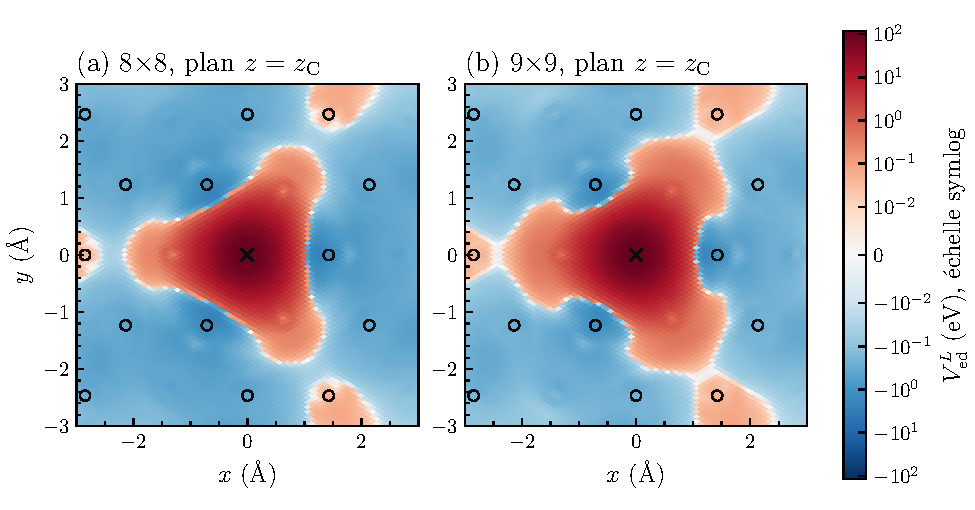
\includegraphics[width=\textwidth]{figures/fig_Ved_zoom.pdf}
    \caption[Potentiel de défaut local au voisinage de la lacune pour deux tailles de super-cellule]{Potentiel de défaut local $V_\text{ed}^\text{L}$ dans le plan du graphène $(z=z_\text{C})$ au voisinage de la lacune, représentée par une croix, pour les super-cellules (a) $8\times 8$ et (b) $9\times 9$. L'échelle est symétrique logarithmique et linéaire entre $\pm 10^{-2}$ eV. Nous voyons une différence qualitative de la forme et de l'orientation des lobes du potentiel de défaut entre les deux tailles de super-cellules. Les deux super-cellules partagent les paramètres de calcul et la
    géométrie non relaxée décrits dans cette section ; seule la divisibilité de la taille $N$ par trois, et donc l'inclusion ou non des points $K$ et $K'$ dans l'échantillonnage, les distingue.}
    \label{fig:Ved_zoom}
\end{figure}
Une grille qui n'échantillonne pas ces états décrit effectivement un isolant ou un semi-conducteur. Nous distinguons alors deux familles de super-cellules : celles avec $N$ divisible par trois qui incluent les points $K$ et $K'$ et l'autre famille. Des différences quantitatives et qualitatives sont illustrées au tableau~\ref{tab:échantillonnage} et à la figure~\ref{fig:Ved_zoom}.

D'abord, la troisième colonne du tableau~\ref{tab:échantillonnage} montre le déplacement du niveau de Fermi $\Delta E_F$ à la création de la lacune. Nous observons que le déplacement en valeur absolue est d'au plus $21~$meV pour la famille qui inclut les points $K$ et $K'$. Les tailles de l'autre famille obtiennent systématiquement des déplacements de l'ordre de quelques centaines de meV, ce qui signale qu'il y a bien une différence physique entre ces deux familles. Un autre indice se trouve dans la quatrième colonne de ce tableau qui illustre la moyenne du potentiel local de la lacune $\bar{V}_\text{ed}^\text{L}(a_\text{CC})$ sur un cercle de rayon $a_\text{CC}=1.42$~\AA~(la distance carbone-carbone dans le graphène) centré sur la lacune. Nous voyons aussi ici une différence quantitative entre les deux familles de tailles de super-cellules : les ordres de grandeur ainsi que le signe diffèrent. Enfin, la figure~\ref{fig:Ved_zoom} illustre le potentiel local de la lacune dans le plan du graphène au voisinage de la lacune qui est représentée par une croix. Les deux familles y sont représentées : en (a) la super-cellule $8\times 8$ qui n'inclut pas les points $K$ et $K'$ et en (b) la super-cellule $9\times 9$ qui les inclut. Nous pouvons voir une différence qualitative de la forme et de l'orientation des lobes du potentiel local au voisinage de la lacune entre les deux familles.

Toutes les super-cellules partagent les mêmes paramètres de calcul et la même géométrie non relaxée (hormis la position exacte du défaut). Seule la divisibilité de la taille $N$ par trois, et donc l'inclusion ou non des points $K$ et $K'$ dans l'échantillonnage, les distingue. Ainsi, nous ne retenons que la famille incluant les points $K$ et $K'$, dont la super-cellule $9\times 9$ sert de référence et les $6\times 6$ et $12\times 12$ servent de contrôle de convergence. L'autre famille, qui n'inclut pas les points $K$ et $K'$, est conservée comme contrôle des artefacts d'échantillonnage.

\bloc{Remplissage par zéros}

Nous vérifions ici la validité de la technique de remplissage par zéros. Celle-ci est exacte si le potentiel est identiquement nul à la frontière de la super-cellule et introduit une approximation autrement. La figure~\ref{fig:Ved} (a,b) montre le potentiel de défaut local dans le plan du graphène pour les super-cellules $5\times 5$ et $9\times 9$ et la figure~\ref{fig:Ved} (c) montre sa moyenne dans le plan, excluant un rayon de $0.5$~\AA~autour de chaque atome où la réorganisation autocohérente de la densité de charge rend le potentiel abrupt et la moyenne sensible à la grille, en fonction de la distance au site de la lacune pour les six tailles. Le site de la lacune, dépourvu d'atome, n'est pas exclu de cette moyenne.
\begin{figure}[htbp]
    \centering
    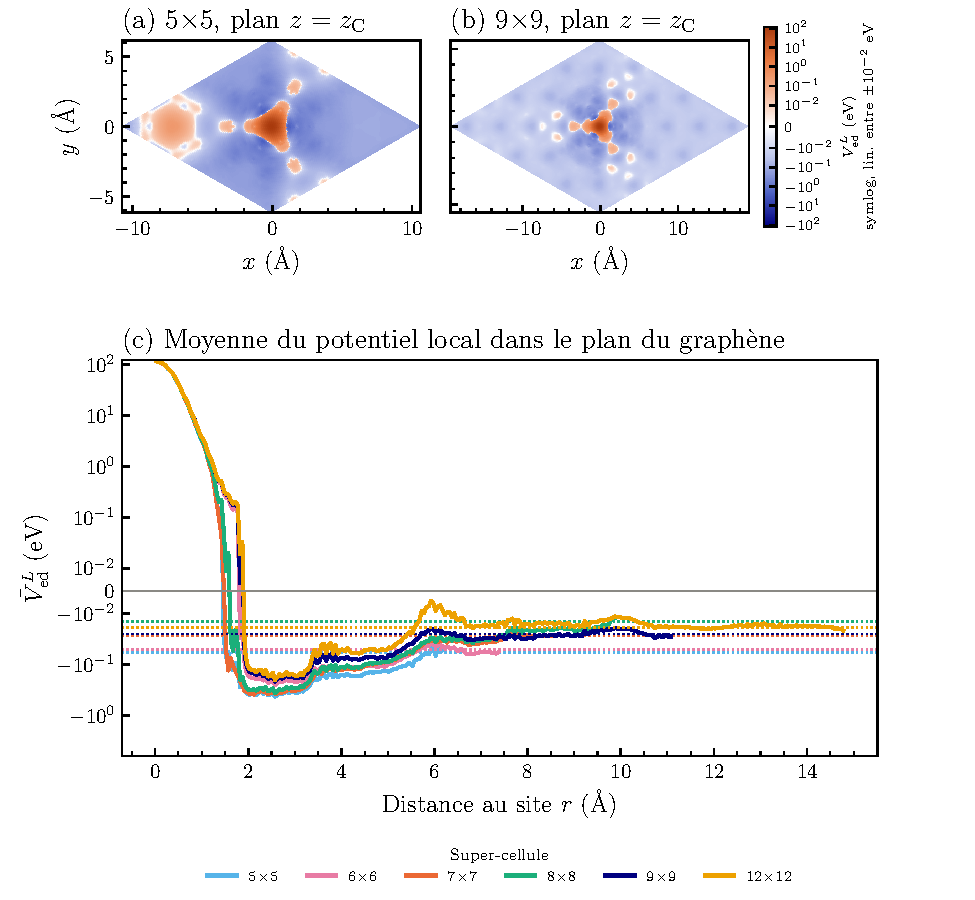
\includegraphics[width=\textwidth]{figures/fig_Ved.pdf}
    \caption[Potentiel de défaut local d'une lacune dans le graphène.]{Potentiel de défaut local $V_\text{ed}^\text{L}$ de la lacune. (a,b) Dans le plan du graphène ($z=z_\text{C}$), pour les super-cellules $5\times 5$ et $9\times 9$ avec une échelle de couleur symétrique logarithmique, linéaire entre $\pm 10 ^{-2}$ eV. Notons la zone positive au coin de la super-cellule $5\times 5$ en (a), absente en (b), qui représente l'interaction de la lacune avec ses images périodiques. (c) Moyenne du potentiel local dans le plan du graphène $\bar V_\text{ed}^\text{L}$, excluant un rayon de $r_\text{at} = 0.5$~\AA~autour des c\oe urs atomiques, pour les six tailles de super-cellules. Chaque courbe s'arrête à la demi-largeur de la super-cellule.}
    \label{fig:Ved}
\end{figure}
Le potentiel de la lacune est dominé par un c\oe ur positif répulsif de l'ordre de $10^2$ eV au site de la lacune, où manque le c\oe ur attractif de l'atome supprimé. Le potentiel chute ensuite de trois ordres de grandeur en moins de 2~\AA{}. Toutefois, au-delà, il ne s'annule pas : un fond négatif faible de $10^{-1}$ eV subsiste jusqu'à la frontière de la super-cellule. Ce fond n'est pas un artefact de la référence du potentiel : il subsiste même après la soustraction des moyennes spatiales des potentiels locaux des super-cellules. Il reflète plutôt l'écrantage incomplet propre au graphène, dont la densité d'états s'annule au point de Dirac~\cite{castronetoElectronicPropertiesGraphene2009}. En outre, la super-cellule $5\times 5$ de la figure~\ref{fig:Ved} (a) présente une zone positive de $\sim 0.1$ eV au coin de la boîte qui est le signe de l'interaction de la lacune avec ses propres images périodiques~\cite{freysoldtFirstprinciplesCalculationsPoint2014}. Cette interaction est de l'ordre du fond et complètement absente pour la super-cellule $9\times 9$ de la figure~\ref{fig:Ved} (b). Cela signifie que la super-cellule $5\times 5$ est trop petite pour contenir la lacune, tandis que la $9\times 9$ est suffisante.

Le remplissage par zéros impose $V_\text{ed}^\text{L} = 0$ au-delà de la frontière, où le fond, quoique faible, ne s'annule pas encore. Le potentiel élargi présente alors une discontinuité de l'ordre de $10^{-1}$ eV à la frontière. Trois facteurs contrôlent cette approximation. D'abord, cette discontinuité est petite comparée au centre répulsif du défaut qui domine le couplage : trois ordres de grandeur sous le c\oe ur de la lacune. Ensuite, cette approximation est confinée à la partie locale du couplage, puisque seul le potentiel local est concerné par l'élargissement. Or, nous verrons plus loin dans cette section que c'est la partie non locale qui domine largement le couplage. Finalement, nous verrons dans le prochain paragraphe que le remplissage par zéro préserve l'échelle des éléments de matrice. C'est une approximation maîtrisée, dont l'erreur est bornée.

\bloc{Convention intensive}

Nous vérifions ici la convention intensive de la section~\ref{sec:M_détails}, c'est-à-dire que la matrice de couplage soit indépendante de la taille $N$ de la super-cellule employée. Cela est effectué dans la figure~\ref{fig:M_scaling}, en comparant le maximum de $|M|$ sur toutes les bandes et tous les points $\kv$ en fonction de la taille $N$ des super-cellules. L'exercice est fait d'une part sur les grilles élargies $pN\times pN$ représentées par des cercles, puis, d'autre part, sur les grilles grossières $N\times N$ représentées par des croix. Pour les grilles élargies, le maximum de $|M|$ varie avec une dispersion inférieure à $2~\%$ sur une plage où le nombre de cellules unitaires $N_\text{cells} = N^2$ varie d'un facteur de six. Les éléments de matrice sont bien intensifs avec notre convention. De plus, l'écart entre les grilles grossières et les grilles élargies est pratiquement nul pour $N\geq 7$, ce qui confirme que le remplissage par zéros préserve l'échelle des éléments de matrice. L'écart résiduel à $N=5$ et $6$ n'est pas une anomalie, mais la contrepartie attendue du paragraphe précédent. Pour ces tailles, la super-cellule n'est pas assez grande pour contenir le potentiel de la lacune (figure~\ref{fig:Ved} (a)) et son prolongement par zéros diffère alors réellement de son prolongement périodique. La cohérence des deux diagnostics montre qu'il est critique que la super-cellule contienne l'ensemble du potentiel de défaut pour appliquer notre méthode.
\begin{figure}[htbp]
    \centering
    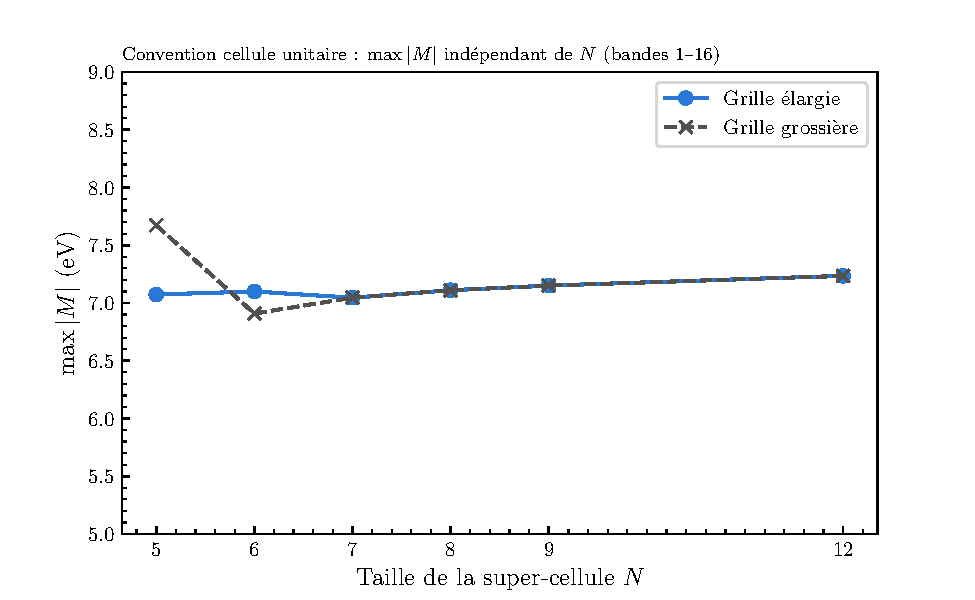
\includegraphics[width=\textwidth]{figures/fig_M_scaling_final.pdf}
    \caption[Vérification de la convention intensive des éléments de matrice.]{Maximum de $|M|$ sur toutes les bandes et les points $\kv$ en fonction de la taille $N$ de la super-cellule. Les croix représentent les grilles grossières tandis que les cercles représentent les grilles élargies. L'indépendance en $N$ vérifie la convention intensive de la section~\ref{sec:M_détails}. L'écart à $N=5$ et $6$ entre les deux types de grilles correspond aux super-cellules qui ne contiennent pas entièrement le potentiel de défaut (figure~\ref{fig:Ved} (a)).}
    \label{fig:M_scaling}
\end{figure}

\bloc{Éléments de matrice au point de Dirac et comparaison avec la littérature}

\begin{figure}[htbp]
    \centering
    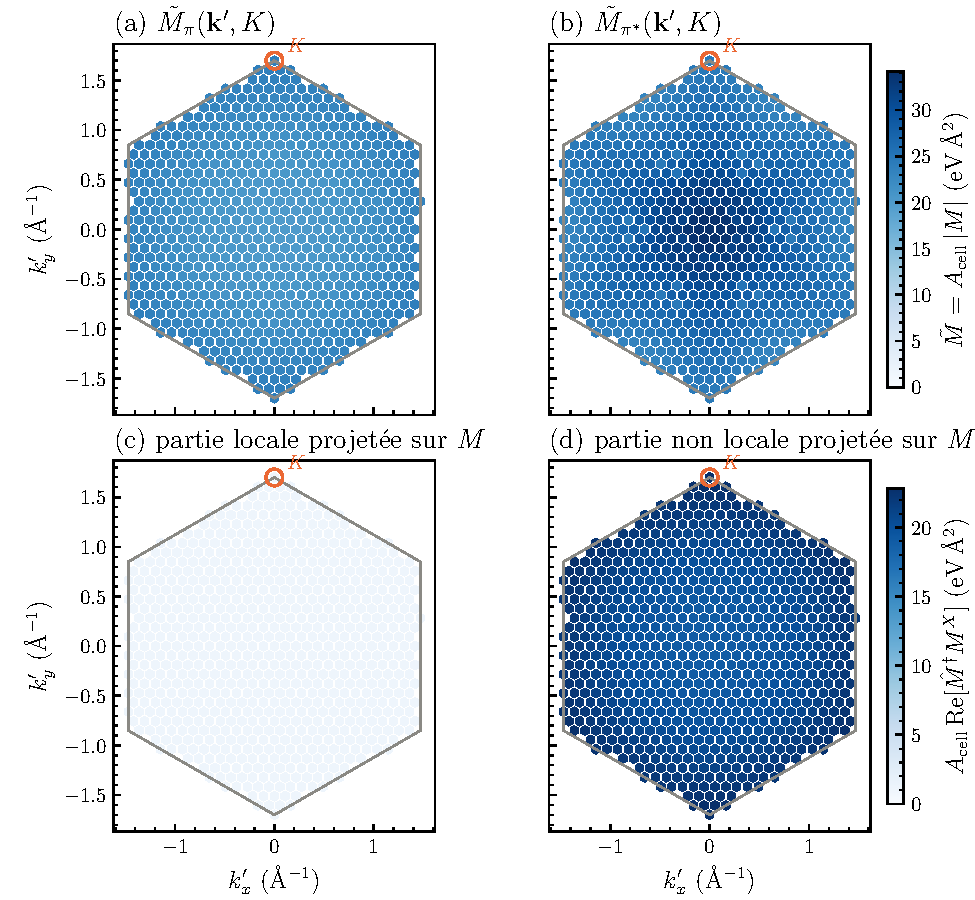
\includegraphics[width=\textwidth]{figures/fig_M_map_final.pdf}
    \caption[Éléments de matrice électron-lacune au point de Dirac.]{Éléments de matrice électron-lacune depuis la paire dégénérée $\pi$--$\pi^*$ au point de Dirac $K$, représenté par un cercle, vers l'état final $\kv'$ sur la grille élargie $27\times 27$ de la super-cellule $9\times 9$. (a,b) Norme invariante $\tilde M_n(\kv')$ en eV\,\AA$^2$ de l'équation~\eqref{eqn:M_tilde} pour l'état final sur la bande $\pi$ (a) et $\pi^*$ (b). (c,d) Contributions locale et non locale à $\tilde M_\pi$ en eV~\AA$^2$, données par l'équation~\eqref{eqn:M_projection}. Leur somme redonne exactement le panneau (a).}
    \label{fig:M_map}
\end{figure}

La figure~\ref{fig:M_map} caractérise le couplage depuis le point de Dirac, où résident les états pertinents pour la diffusion Raman résonante. L'état initial est fixé à $K$ et l'état final $\kv'$ parcourt la zone de Brillouin de la cellule unitaire, échantillonnée sur la grille élargie $27\times 27$ de la super-cellule $9\times 9$. Une subtilité technique impose le choix de la quantité tracée : au point $K$, les bandes $\pi$ et $\pi^*$ sont dégénérées et la diagonalisation numérique retourne une combinaison arbitraire des deux états, de sorte qu'un élément de matrice individuel comme $M_{\pi\pi}(\kv',K)$ n'est pas défini de manière unique. Nous traçons donc le couplage sur la paire dégénérée $\{m_1,m_2\}$
\begin{equation}
    \tilde M_n(\kv') = A_\text{cell}\left[\sum_{i=1}^2\left|M_{n(\kv')m_i}(\kv',K)\right|^2\right]^{1/2},\label{eqn:M_tilde}
\end{equation}
où $A_\text{cell} = 5.27$~\AA$^2$ est l'aire de la cellule unitaire, de sorte que $\tilde M$ s'exprime en eV\,\AA$^2$, et où la bande de l'état final $n(\kv')\in\{\pi,\pi^*\}$ est identifiée en chaque $\kv'$ par son poids orbital $p_z$, ce qui la distingue des bandes $\sigma$ aux croisements. Les panneaux (c,d) décomposent $\tilde M_\pi$ en ses contributions locale et non locale. En rassemblant les deux éléments de matrice en un vecteur complexe $v_i(\kv') = M_{\pi(\kv')m_i}(\kv',K)$, chaque contribution est projetée sur la direction du couplage total
\begin{equation}
    M^\text{X}_\parallel(\kv')= A_\text{cell}\mathrm{Re}\left[\hat v^\dagger(\kv')v^\text{X}(\kv')\right],\label{eqn:M_projection}
\end{equation}
où $\text{X}\in\{\text{L},\text{NL}\}$, $\hat v = v/|v|$ et $v_i^\text{X}= M^\text{X}_{\pi(\kv')m_i}(\kv',K)$. Ces projections sont également invariantes sous le même choix de diagonalisation et leur somme redonne
\begin{equation*}
    \tilde M_{\pi}(\kv') = M^\text{L}_\parallel(\kv') + M^\text{NL}_\parallel(\kv'),
\end{equation*}
par construction.

La carte pour $\tilde M_\pi$ est remarquablement uniforme : elle vaut 23.9 eV\,\AA${^2}$~au point $K$ et ne s'en écarte que peu sur la zone. La carte pour $\tilde M_{\pi^*}$ l'est un peu moins : elle vaut 24.5 eV\,\AA$^{2}$~en $K$ avec un maximum de 34.2 eV\,\AA$^2$~au centre de la zone. Ces valeurs se comparent à celles de la littérature. Nous comparons avec l'article de Kaasbjerg~\cite{kaasbjergAtomisticMatrixTheory2020}, qui rapporte $\sim 70$ eV\,\AA$^2$ pour les éléments intravallée et intervallée d'une lacune dans le graphène (valeur lue sur sa figure 3 qui trace l'élément intrabande individuel $|V_{\kv\kv'}^{nn}|$ avec l'état initial légèrement décalé de $K$ pour contourner la dégénérescence). Son calcul emploie le formalisme PAW (\textit{Projector Augmented Waves}, qui reconstruit les fonctions d'onde tous-électrons à partir d'un calcul à c\oe ur gélé~\cite{blochlProjectorAugmentedwaveMethod1994}) dans le code \texttt{GPAW}, la fonctionnelle d'échange-corrélation LDA et une super-cellule $11\times 11$. L'article indique que la relaxation structurale, mineure pour les défauts des dichalcogénures, est négligée, mais il ne précise pas si ce choix s'étend à son calcul du graphène, où la reconstruction de la lacune n'est précisément pas mineure. Sa convention intensive est identique à la nôtre. L'interprétation physique concorde : il attribue, comme nous, le signe répulsif au c\oe ur attractif manquant de l'atome supprimé. L'amplitude diffère toutefois : en convertissant notre norme sur la paire vers un élément individuel ($\tilde M/\sqrt{2}$ lorsque les éléments de la paire sont comparables, ce que son approximation de potentiel ponctuel suppose), nos valeurs sont inférieures d'un facteur de 3 à 4. Cet écart peut provenir de la fonctionnelle d'échange-corrélation (PBE contre LDA), de la base (ondes planes contre orbitales localisées et PAW), du traitement des électrons de c\oe ur (pseudopotentiel ONCV de type KB contre PAW), et de la relaxation autour du défaut, sans que nous ayons pu l'attribuer à une cause exacte. Les éléments de matrice ne sont toutefois pas des observables : ce sont des quantités intermédiaires dépendantes du formalisme. La comparaison probante se fera au niveau des observables, tel le taux d'amortissement $\Gamma^\text{ed}$ et, à terme, l'intensité Raman résonante.

\bloc{Contributions locales et non locales}

Les panneaux (c,d) de la figure~\ref{fig:M_map} et le tableau~\ref{tab:L_NL} quantifient la décomposition locale/non locale de l'équation~\eqref{eqn:M_projection}. Le résultat est marquant sur la figure : la partie non locale, comprise entre 19 et 23 eV\,\AA$^2$, domine sur toute la zone de Brillouin, tandis que la partie locale ne dépasse jamais $1.3$ eV\,\AA$^2$. Le tableau~\ref{tab:L_NL}
suit ce rapport pour les six tailles de super-cellules, en calculant la demi-trace du bloc dégénéré au point de Dirac
\begin{equation}
    \bar M^\text{X}(K) = \tfrac{1}{2}\mathrm{Re}\mathrm{Tr}M^\text{X}(K,K),\label{eqn:M_bar}
\end{equation}
qui est invariante, comme la norme, sous les rotations unitaires de la paire. La deuxième colonne montre que la partie non locale est stable à 3.10 eV (avec variations de quelques $10^{-3}$ eV) tandis que la première colonne montre que la partie locale décroît de 0.42 eV à 0.08 eV. La partie locale, écrantée, porte toute la dépendance en taille de la super-cellule et la partie non locale en est indépendante. Notons que le panneau (a) de la figure~\ref{fig:M_map} et les deux premières colonnes du tableau~\ref{tab:L_NL} ne rapportent pas la même quantité au point $K$ : la figure rapporte $ \tilde M_\pi(K)=23.9$ eV~\AA$^2$ et le tableau rapporte $A_\text{cell}\bar M(K)=17.1$ eV~\AA$^2$ pour $N=9$, où $\bar M = \bar M^\text{L}+\bar M^\text{NL}$. L'écart vient de l'élément interbande $\pi\leftrightarrow\pi^*$ que la norme inclut alors que la trace l'ignore. La dernière colonne du tableau, qui rapporte le rapport des normes de Frobenius $\langle |M^\text{NL}|\rangle/\langle |M^\text{L}|\rangle$ sur le sous-espace $\pi$--$\pi^*$ et toutes les paires $(\kv',\kv)$ de la BZ échantillonnée sur la grille élargie, montre que la partie non locale domine sur toute la BZ et non seulement à $K$.
\begin{table}[htbp]
    \centering
    \caption[Contributions locale et non locale
     à la matrice de couplage électron-défaut.]{Contributions locale et non locale à la matrice de couplage. Les deux premières colonnes rapportent la demi-trace invariante de l'équation~\eqref{eqn:M_bar} pour les deux parties au point de Dirac $K$ pour les six tailles de super-cellule. La dernière colonne donne le rapport des normes de Frobenius $\langle |M^\text{NL}|\rangle/\langle |M^\text{L}|\rangle$ sur le sous-espace $\pi$--$\pi^*$ et toutes les paires $(\kv',\kv)$ de la grille élargie.}
    \label{tab:L_NL}
    \begin{tabular}{c c c c}
        \hline\hline
        $N$ & $\bar M^\text{L}(K)$ (eV) & $\bar M^\text{NL}(K)$ (eV) & NL/L toute la BZ \\
        \hline
        5  & 0.421 & 3.100 & 6.5 \\
        6  & 0.315 & 3.103 & 9.1 \\
        7  & 0.214 & 3.101 & 12.7 \\
        8  & 0.168 & 3.101 & 16.4 \\
        9  & 0.140 & 3.103 & 20.4 \\
        12 & 0.078 & 3.103 & 36.3 \\
        \hline\hline
    \end{tabular}
\end{table}
Cette différence a une origine simple : la partie locale est une différence de potentiels autocohérents, dans laquelle les réponses d'Hartree et d'échange-corrélation écrantent le trou de potentiel créé par la lacune, tandis que la partie non locale est le retrait des projecteurs de Kleinman-Bylander de l'atome absent, que rien n'écrante. Cette séparation est due à notre choix de pseudo-potentiels et n'a pas de signification physique en soi : seule la somme des deux parties en a une. Cependant, elle a une conséquence pratique pour notre approche : le remplissage par zéros est encore plus justifié, même si le potentiel local n'est pas exactement nul à la frontière puisqu'il n'affecte que la partie locale représentant au plus $13~\%$ du couplage pour la plus petite super-cellule et moins de $5~\%$ pour la référence $9\times 9$.

\bloc{Localisation dans la base de Wannier}

La figure~\ref{fig:M_locality} présente la norme de Frobenius des blocs $M_{ij}(\Rv,\bm 0)$ en fonction de la distance $R$ à la lacune située à l'origine après le recentrage, pour les quatre super-cellules $N=5, 8, 9, 12$ sur la grille élargie obtenue par remplissage par zéros et, pour $N=5, 8$, sur la grille grossière $N\times N$.
\begin{figure}[htbp]
    \centering
    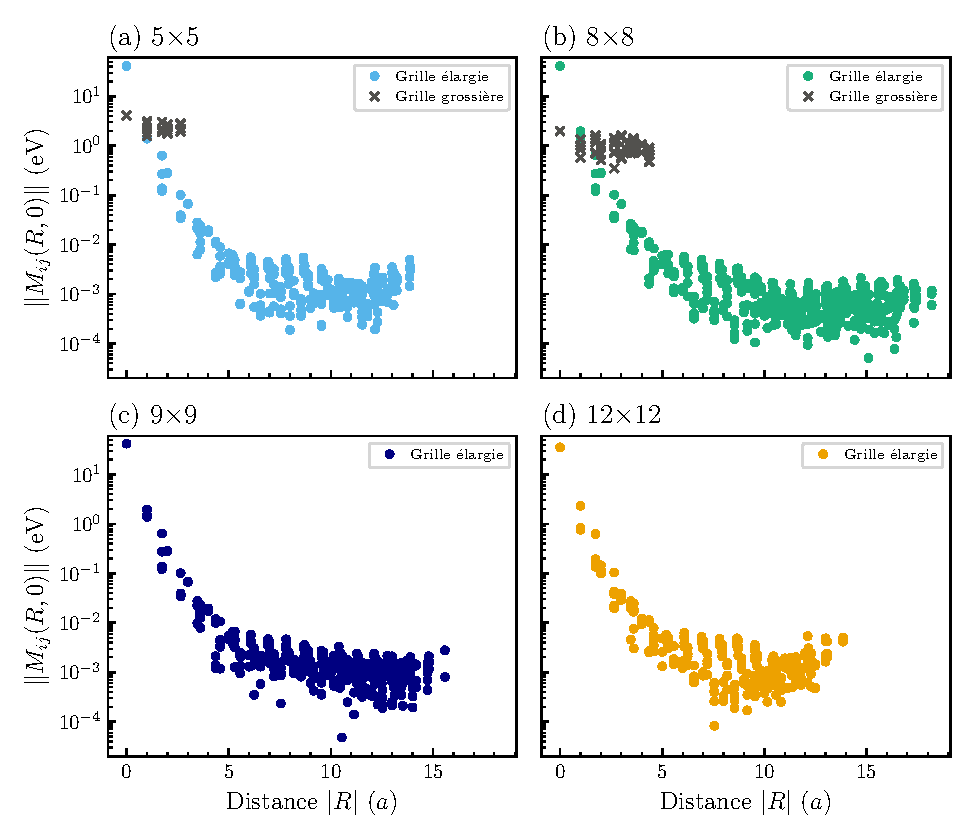
\includegraphics[width=\textwidth]{figures/fig_locality_final.pdf}
    \caption[Localisation de la matrice de couplage électron-lacune dans la base des fonctions de Wannier.]{Norme de Frobenius des blocs $M_{ij}(\Rv,\bm 0)$ de la matrice de couplage électron-lacune dans la base des fonctions de Wannier, où la lacune a été ramenée à l'origine par recentrage, en fonction de
    la distance $R$ en unités du paramètre de maille, pour les
    super-cellules $N = 5, 8, 9, 12$. Les cercles (a,b,c,d) représentent les grilles élargies $pN\times pN$ et les croix identifient les grilles grossières $N\times N$ (a,b).}
    \label{fig:M_locality}
\end{figure}
D'une part, les grilles grossières (représentées par des croix aux panneaux (a,b)) ne donnent pas lieu à une décroissance rapide. D'autre part, sur les grilles élargies (représentées par des cercles aux panneaux (a,b,c,d)) le poids chute de quatre ordres de grandeur sur les cinq premières cellules unitaires avant d'atteindre un plancher de $10^{-4}$ eV. C'est la décroissance rapide attendue des éléments de matrice dans la base des fonctions de Wannier pour un défaut localisé dans l'espace réel. Cette différence entre les deux types de grilles est un effet de repliement spectral (de l'anglais \textit{aliasing}). La transformée~\eqref{eqn:M_wannier} sur une grille de $N\times N$ points ne produit que $N^2$ vecteurs $\Rv$ et tout poids situé au-delà de cette boîte est replié sur les mailles disponibles, ce qui étale artificiellement le poids et masque la localisation. Les grilles élargies de $pN\times pN$ points disposent de $p^2$ fois plus de vecteurs $\Rv$ et rendent la localisation manifeste. Le remplissage par zéros est donc indispensable à l'interpolation de Wannier : sans lui, la représentation réelle du couplage n'est pas localisée et aucune troncature n'est légitime.

\begin{table}[htbp]
    \centering
    \caption[Erreur de troncature sur les éléments de
    matrice interpolés.]{Écart relatif maximal entre les éléments de
    matrice interpolés sur une grille fine $60\times60$ avec troncature de
    la somme~\eqref{eqn:M_interp} à $R',R \le R_\text{cut}$, où $R$ et $R'$ sont des normes euclidiennes d'indices réduits, et ceux
    obtenus avec toutes les cellules unitaires de la représentation réelle, pour les
    super-cellules $9\times9$ et $12\times12$ sur les valeurs singulières
    des blocs $\pi$--$\pi^*$ et sur les éléments
    diagonaux $M_{nn}(\kv,\kv)$. La deuxième colonne donne le nombre de
    cellules unitaires retenues.}
    \label{tab:rcut_M}
    \begin{tabular}{c c cc cc}
        \hline\hline
        & & \multicolumn{2}{c}{$9\times9$} & \multicolumn{2}{c}{$12\times12$} \\
        $R_\text{cut}$ & Nombre de cellules & $\pi$--$\pi^*$ & diag. & $\pi$--$\pi^*$ & diag. \\
        \hline
        0 & 1   & 41~\%    & 41~\%    & 97~\%    & 73~\%    \\
        1 & 5   & 24~\%    & 17~\%    & 18~\%    & 18~\%    \\
        2 & 13  & 7.2~\% & 4.8~\% & 12~\%    & 12~\%    \\
        3 & 29  & 2.6~\% & 2.1~\% & 3.1~\% & 2.4~\% \\
        4 & 49  & 1.6~\% & 1.4~\% & 1.7~\% & 1.5~\% \\
        5 & 81  & 1.1~\% & 1.1~\% & 1.3~\% & 1.2~\% \\
        6 & 113 & 1.0~\% & 1.0~\% & 1.2~\% & 1.1~\% \\
        \hline\hline
    \end{tabular}
\end{table}
Le tableau~\ref{tab:rcut_M} mesure l'effet de la troncature sur les éléments de matrice interpolés. À $R_\text{cut} =3$ (norme euclidienne des indices réduits), soit 29 cellules unitaires, l'écart aux éléments de matrice obtenus avec toutes les mailles est de 2 à 3~\% autant pour les bandes $\pi$ et $\pi^*$ que pour les éléments diagonaux. Au-delà, la décroissance ralentit nettement : l'écart n'est plus que de 1.6~\% à $R_\text{cut}=4$ et plafonne autour de $1~\%$ à $R_\text{cut}=6$, avec 113 cellules unitaires. Cet écart résiduel est la contribution cumulée des centaines de mailles éloignées de valeurs individuellement inférieures à $10^{-3}$ de l'élément sur le site. Réduire cet écart à zéro exigerait un rayon de coupure bien supérieur pour un coût computationnel bien plus grand. Ce test est croisé avec celui à la section~\ref{sec:T_results} pour la convergence en $R_\text{cut}$ du taux d'amortissement. Nous retenons $R_\text{cut}=3$ pour la production : la section~\ref{sec:T_results} vérifie que l'erreur de $2$ à $3~\%$ sur les éléments de matrice se traduit par un effet négligeable sur le taux d'amortissement, l'observable physique visée.

\bloc{Autres vérifications}

Le tableau~\ref{tab:tests_M} rassemble toutes les vérifications de la chaîne de calcul de la matrice $M$. Le test le plus contraignant porte sur la machinerie de calcul elle-même : en l'appliquant au potentiel de Kohn-Sham convergé de la super-cellule parfaite (et en ajoutant l'énergie cinétique) plutôt qu'au potentiel de défaut, elle doit reconstruire la matrice Hamiltonienne de Kohn-Sham dans la base de ses états propres, c'est-à-dire retourner les valeurs propres $\varepsilon_{n\kv}$ sur la diagonale et zéro ailleurs. La figure~\ref{fig:ks_reconstruction} montre les résultats pour les six tailles.
\begin{figure}[htbp]
    \centering
    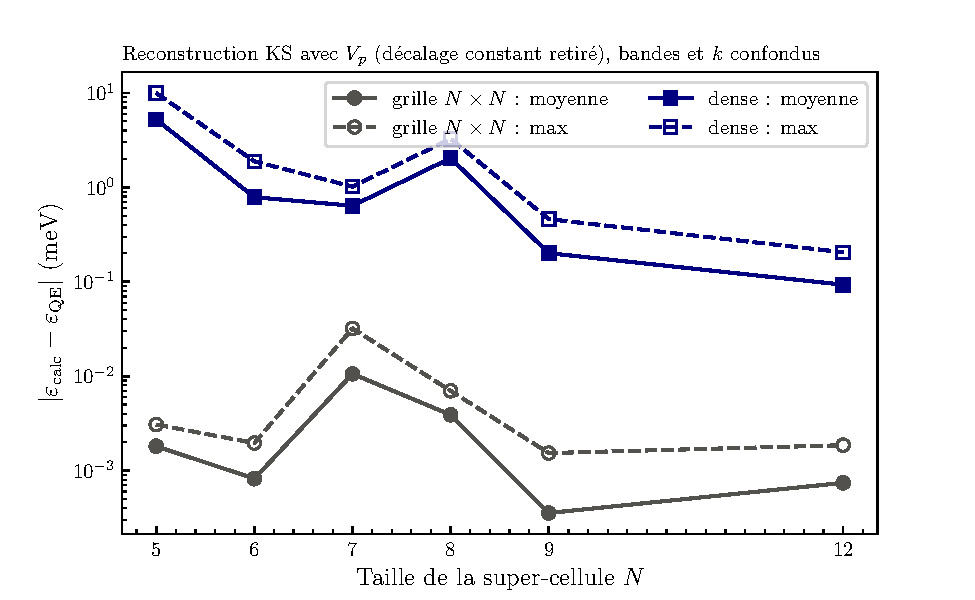
\includegraphics[width=\textwidth]{figures/fig_ks_reconstruction.pdf}
    \caption[Reconstruction des valeurs propres de Kohn-Sham.]{Écart
    entre les valeurs propres de Kohn-Sham reconstruites par la chaîne
    d'évaluation des éléments de matrice, appliquée au potentiel de la
    super-cellule parfaite, et celles de \texttt{QuantumESPRESSO}.
    La moyenne et le maximum sont sur toutes les bandes et tous les points $\kv$, après le retrait d'un décalage constant entre les deux références d'énergie. L'exercice est fait pour les grilles $N\times N$, où la densité convergée est la même pour les états et le potentiel, et pour les grilles élargies $pN\times pN$, où la densité autocohérente est différente.}
    \label{fig:ks_reconstruction}
\end{figure}
Pour les grilles grossières $N\times N$, où les états de Bloch et le potentiel proviennent du même calcul autocohérent, les valeurs propres de \texttt{QuantumESPRESSO} sont reproduites à 2--32 $\mu$eV près et les éléments hors diagonaux sont inférieurs à $10^{-6}$ en valeur relative. Ce test valide contre une référence indépendante du code le repliement des vecteurs $\Gv$, les facteurs de forme, les phases atomiques, la normalisation et les préfacteurs communs aux deux parties de la matrice de couplage. Seule la soustraction des deux super-cellules lui échappe. Sur les grilles élargies $pN\times pN$, l'écart atteint 0.2 à 10 meV, ce qui est attendu puisque les états de Bloch proviennent de la cellule unitaire avec la grille élargie $pN\times pN$ tandis que le potentiel vient du calcul de la super-cellule, dont l'échantillonnage à $\Gamma$ équivaut à une grille $N\times N$. Les densités autocohérentes ne sont donc pas identiques, et le potentiel n'est pas exactement celui dont les états de Bloch sont les états propres. Cette incohérence est inhérente à toute approche par super-cellule et ne pose pas de problème pour notre méthode.

Les autres tests sont des vérifications de cohérence interne. L'hermiticité des matrices de couplage est respectée à $10^{-14}$. Le remplissage par zéros préserve les coefficients de Fourier aux points coïncidents à $10^{-15}$. Le passage de 16 à 20 bandes modifie les éléments de matrice des bandes retenues de $10^{-7}$ en valeur relative. La transformée de Fourier $\kv\to\Rv\to\kv$ reproduit les éléments de matrice de départ à $10^{-14}$ près, et la transformée aller-retour Bloch$\to$Wannier$\to$Bloch (les équations~\eqref{eqn:M_wannier} et~\eqref{eqn:M_interp}) évaluée aux points de la grille grossière elle-même, à $10^{-15}$ près. Le seul écart supérieur au bruit numérique, de $10^{-3}$, apparaît en comparant les éléments de matrice des grilles grossières et élargies aux points $\kv$ communs. Cet écart a la même origine que l'écart de reconstruction sur les grilles élargies c'est-à-dire la différence entre les deux densités autocohérentes, et non la chaîne de calcul de $M$.
\begin{table}[htbp]
    \centering
    \small
    \setlength{\tabcolsep}{2pt}
    \caption[Vérifications de la chaîne de calcul de la matrice de
    couplage.]{Vérifications de la chaîne de calcul de la matrice $M$ : les tests et la quantité qu'ils contrôlent, la valeur obtenue et le seuil d'acceptation. Sauf mention contraire la valeur est celle de la super-cellule de référence $9\times9$ ; les reconstructions de Kohn-Sham sont données en fourchette sur les six tailles et le test de convention intensive porte par construction sur l'ensemble des tailles.}
    \label{tab:tests_M}
    \begin{tabular}{l l l l}
        \hline\hline
        Test & Quantité & Valeur & Seuil \\
        \hline
        Reconstruction KS, grille $N\times N$ & $\max|\varepsilon_\text{calc}-\varepsilon_\text{QE}|$ & 2--32~$\mu$eV & --- \\
        \quad éléments hors diagonaux & rel. à $\max|\varepsilon|$ & $\le 1.3\times10^{-6}$ & --- \\
        Reconstruction KS, grille élargie & $\max|\varepsilon_\text{calc}-\varepsilon_\text{QE}|$ & 0.2--10~meV & --- \\
        Hermiticité ($M$ élargi) & $\max|M-M^\dagger|/\max|M|$ & $\le 4\times10^{-14}$ & $10^{-12}$ \\
        Remplissage, coefficients coïncidents & $\max|\Delta M^\text{L}|/\max|M^\text{L}|$ & $1.3\times10^{-15}$ & $10^{-10}$ \\
        Remplissage, points $\kv$ communs & écart rel. valeurs singulières & $1.2\times10^{-3}$ & $2\times10^{-3}$ \\
        16 $\to$ 20 bandes & écart rel. valeurs singulières & $1.2\times10^{-7}$ & $10^{-5}$ \\
        Fourier $\kv\to\Rv\to\kv$ & $\max|\Delta M|/\max|M|$ & $2.4\times10^{-14}$ & $10^{-12}$ \\
        Bloch$\to$Wannier$\to$Bloch & écart rel. valeurs singulières & $1.3\times10^{-15}$ & $10^{-12}$ \\
        Convention intensive & $(\max-\min)/\text{moy.}$ de $\max|M|$ sur $N$ & $1.1\times10^{-2}$ & $5\times10^{-2}$ \\
        \hline\hline
    \end{tabular}
\end{table}

Au terme de cette section, nous disposons de la matrice de couplage électron-défaut $M$ du graphène, calculée à partir des premiers principes sur la grille de la super-cellule, validée contre une référence indépendante, et interpolable sur une grille de vecteurs d'onde arbitrairement dense grâce aux fonctions de Wannier. Ce sont ces éléments de matrice qui entrent directement dans les amplitudes de diffusion \textit{phonon-défaut} du chapitre~\ref{chap:Raman}. Il reste à en extraire la seconde quantité annoncée en introduction : le taux d'amortissement $\Gamma_{n\kv}^\text{ed}$, qui décrit l'effet cumulé d'une collection de défauts sur la durée de vie des états électroniques. La section suivante établit le formalisme qui relie la matrice $M$ à ce taux, puis l'applique au graphène avec la même rigueur de vérification.

\section{Théorie de la perturbation à plusieurs corps pour les défauts}\label{sec:mbt_défaut}
Dans cette section, nous détaillons comment utiliser la théorie de la perturbation à plusieurs corps dans le contexte de l'interaction électron-défaut pour relier les éléments de matrice de couplage de la section précédente à la \textit{self}-énergie électronique due à la présence de défauts dans un matériau. Nous commençons avec le cas le plus simple où un seul et unique défaut est présent dans le matériau. Dans ce cas, le problème peut être résolu exactement dans le formalisme de la matrice $T$~\cite{bruusManyBodyQuantumTheory2004}. Ensuite, nous généralisons au cas d'un grand nombre de défauts répartis aléatoirement pour simuler un matériau réel. Les quantités mesurables par l'expérience ne dépendent pas de la réalisation microscopique des défauts et sont des moyennes sur toutes les positions des défauts. Cette moyenne ne peut pas être évaluée exactement, d'où l'utilité de la théorie de la perturbation.

\subsection{Un défaut et la matrice $T$}\label{sec:mbt_T}

Commençons par le cas idéal où il n'y a qu'un seul défaut présent dans le matériau et ignorons toutes les autres perturbations. Supposons que le problème électronique a été résolu par la DFT dans le système parfait. Le couplage entre les électrons du système et le défaut se fait par l'entremise de l'Hamiltonien de couplage électron-défaut, et nous travaillons maintenant à température finie c'est-à-dire dans l'ensemble grand canonique, de sorte que l'Hamiltonien du système est
\begin{equation}
    \hat{H}-\mu\hat{N} = \hat{H}_\text{e}+\hat{H}_\text{ed} = \sum_{n\kv}\xi_{n\kv}\hat{c}^\dag_{n\kv}\hat{c}_{n\kv}+\sum_{nm}\sum_{\kv\kv'}M_{mn}(\kv',\kv)\hat{c}^\dag_{m\kv'}\hat{c}_{n\kv},\quad\xi_{n\kv} \equiv \varepsilon_{n\kv}-\mu
\end{equation}
où la matrice $M_{mn}(\kv',\kv)=\matrixel{\psi_{m\kv'}}{V_\text{ed}(\rv)}{\psi_{n\kv}}$ représente physiquement l'amplitude de probabilité qu'un électron dans l'état $\ket{\psi_{n\kv}}$ diffuse vers l'état $\ket{\psi_{m\kv'}}$ via le potentiel $V_\text{ed}(\rv)$ induit par le défaut dans le matériau, $\xi_{n\kv}\equiv\varepsilon_{ n\kv}-\mu$ et $\mu$ est le potentiel chimique. Nous souhaitons employer la méthode de la théorie de la perturbation pour résoudre ce problème. Notre objectif est de déterminer la fonction de Green de Matsubara à température finie ; une fois celle-ci calculée, la grande majorité des propriétés physiques mesurables peuvent être extraites de cette fonction. Dans le formalisme de Matsubara, nous travaillons avec un temps imaginaire $\tau\in[0,\beta]$, où $\beta=1/k_BT$ est l'inverse de la température et la fonction de Green est généralement calculée dans la représentation d'interaction en mécanique quantique~\cite{mahanManyParticlePhysics2000}
\begin{equation}
    \mathcal{G}_{mn}(\tau'-\tau) = -\frac{{}_0\langle\mathcal{T}_\tau\hat{c}_m(\tau')S(\beta,0)\hat{c}
    _n^\dag(\tau)\rangle_0}{{}_0\langle S(\beta,0)\rangle_0}.\label{eqn:G_formel}
\end{equation}
Ici, les indices $m$ et $n$ de l'équation~\eqref{eqn:G_formel} sont des indices composés de bande et de vecteur d'onde, $m\equiv(m\kv')$ et $n\equiv(n\kv)$, ${}_0\langle\dots\rangle_0$ est une moyenne thermique par rapport à l'Hamiltonien non perturbé $\hat{H}_\text{e}$, $\mathcal{T}_\tau$ est l'opérateur d'ordonnancement dans le temps imaginaire, la dépendance en temps imaginaire des opérateurs $\hat{O}(\tau)$ est obtenue dans la représentation de l'interaction (donc déterminée par $\hat{H}_\text{e}$) et la matrice $S(\beta, 0)$ inclut les effets de couplage entre les électrons et le défaut et est définie formellement par
\begin{equation}
    S(\beta, 0) = \mathcal{T}_\tau\exp[-\int_0^\beta d\tau\,\hat{H}_\text{ed}(\tau)] = \sum_{p=0}^\infty\frac{(-1)^p}{p!}\int_0^\beta d\tau_1\dots\int_0^\beta d\tau_p\mathcal{T}_\tau\left[\hat{H}_\text{ed}(\tau_1)\cdots\hat{H}_\text{ed}(\tau_p)\right].\label{eqn:S}
\end{equation}
Pour calculer la fonction de Green de l'équation~\eqref{eqn:G_formel}, nous devons développer la matrice $S$ à l'aide de l'équation~\eqref{eqn:S} puis évaluer les moyennes thermiques. Comme ces moyennes sont faites par rapport à l'Hamiltonien libre $\hat{H}_\text{e}$, qui est quadratique dans les opérateurs de création et d'annihilation, elles peuvent être évaluées avec le théorème de Wick. Cependant, cette approche souffre du même problème que l'application de la théorie de la perturbation dans le cadre de la spectroscopie Raman : il n'est pas trivial d'énumérer tous les termes qui découlent du développement de la matrice $S$. Pour remédier à ce problème, nous employons à nouveau des diagrammes de Feynman, avec les règles de la figure~\ref{fig:règles_Raman}. En théorie, nous devons développer la matrice $S$ au numérateur et au dénominateur de l'équation~\eqref{eqn:G_formel} simultanément, ce qui devient rapidement problématique. En pratique, le théorème des amas connexes (de l'anglais \textit{linked-cluster theorem}) stipule que les diagrammes engendrés par le développement de la matrice $S$ au dénominateur annulent exactement les diagrammes déconnectés du développement au numérateur. Cela simplifie considérablement la tâche. Toute cette machinerie est présentée en détail dans l'annexe~\ref{annexe:défauts} et nous reprenons seulement les étapes importantes ici.

Le résultat central de cette annexe est que la fonction de Green de Matsubara pour des électrons en interaction avec un seul défaut satisfait une équation de Dyson qui est illustrée diagrammatiquement dans la figure~\ref{fig:G_Dyson}.
\begin{center}
    \vspace{0.5\baselineskip}
    \input{tikz/dyson_serie.tex}
    \captionof{figure}{Équation de Dyson pour la fonction de Green de Matsubara électronique en présence d'un défaut.}
    \label{fig:G_Dyson}
    \vspace{0.5\baselineskip}
\end{center}
Cette équation de Dyson est plus généralement réécrite en employant la matrice $T$ dans le contexte de la diffusion sur des défauts. Cette matrice $T$ est définie diagrammatiquement à la figure~\ref{fig:T_matrice} et joue un rôle similaire à la \textit{self}-énergie électronique.
\begin{center}
    \vspace{0.5\baselineskip}
    \input{tikz/matrice_T.tex}
    \captionof{figure}[Expression diagrammatique de la matrice $T$ pour la diffusion sur un seul défaut.]{Expression diagrammatique de la matrice $T$ pour la diffusion sur un seul défaut. La première ligne donne le développement complet, la deuxième la forme récursive.}
    \label{fig:T_matrice}
    \vspace{0.5\baselineskip}
\end{center}
À l'aide de la matrice $T$, l'équation de Dyson pour la fonction de Green prend la forme donnée diagrammatiquement à la figure~\ref{fig:dyson_T}.
\begin{center}
    \vspace{0.5\baselineskip}
    \input{tikz/dyson_matrice_T.tex}
    \captionof{figure}[Série de Dyson pour la fonction de Green en présence d'un seul défaut, via la matrice $T$.]{Série de Dyson pour la fonction de Green de Matsubara électronique en présence d'un seul défaut, exprimée en fonction de la matrice $T$. Les temps $\tau_1$ et $\tau_2$ sont intégrés.}
    \label{fig:dyson_T}
    \vspace{0.5\baselineskip}
\end{center}
En traduisant ces diagrammes à l'aide des règles de Feynman, la matrice $T$ de la figure~\ref{fig:T_matrice} s'écrit
\begin{equation}
    T = M + M\mathcal{G}^{(0)}T,\label{eqn:T_chap}
\end{equation}
où les produits sont matriciels sur les indices $(n\kv)$ et convolutifs en temps imaginaire, et la fonction de Green de la figure~\ref{fig:dyson_T} devient
\begin{equation}
    \mathcal{G} = \mathcal{G}^{(0)}+\mathcal{G}^{(0)}T\mathcal{G}^{(0)}.\label{eqn:G_chap}
\end{equation}
Les convolutions en temps imaginaire se démêlent dans l'espace des fréquences de Matsubara fermioniques $i\omega_j$, défini à l'annexe~\ref{annexe:défauts} dans l'équation~\eqref{eqn_G_tau}, où elles deviennent de simples produits. La quantité $\mathcal{G}^{(0)}$ est la fonction de Green de Matsubara pour le système non perturbé, soit en l'absence de défauts. Elle est connue analytiquement et prend la forme
\begin{equation}
    \mathcal{G}^{(0)}_{n\kv}(i\omega_j) = \frac{1}{i\omega_j-\xi_{n\kv}}.
\end{equation}
Comme le défaut est statique, $M$ ne dépend pas de la fréquence et l'équation~\eqref{eqn:T_chap} se résout par une inversion de matrice à chaque fréquence
\begin{equation}
    T(i\omega_j) = \left[\mathbb{I}-M\mathcal{G}^{(0)}(i\omega_j)\right]^{-1}M.
\end{equation}
Une fois la matrice $T$ calculée, nous pouvons calculer la fonction de Green qui prend la forme explicite
\begin{equation}
    \mathcal{G}_{mn}(\kv',\kv;i\omega_j) =\delta_{mn}\delta_{\kv\kv'}\mathcal{G}^{(0)}_{n\kv}(i\omega_j)+\mathcal{G}_{m\kv'}^{(0)}(i\omega_j)T_{mn}(\kv',\kv; i\omega_j)\mathcal{G}_{n\kv}^{(0)}(i\omega_j),
\end{equation}
dans l'espace des fréquences de Matsubara. Notons que nous avons ici une expression analytique \textit{exacte} pour la fonction de Green : le problème est résolu exactement. Ceci ne devrait pas être trop surprenant, car il s'agit d'un problème à un corps. Notons également que le formalisme de la matrice $T$ inclut les effets du défaut sur les électrons à tous les ordres de la théorie de la perturbation. Cela est particulièrement intéressant pour les défauts considérés dans ce mémoire, les lacunes, qui induisent un potentiel de défaut si fort qu'il n'est pas justifié de tronquer la série de Dyson à un ordre fini. Le formalisme de la matrice $T$ demeure valide dans tous les régimes de force de potentiel de défaut.
Enfin, notons que les quantités physiques mesurables sont les fonctions dites \textit{retardées}, définies
sur l'axe des fréquences réelles, tandis que nous avons des expressions pour les quantités sur l'axe des fréquences imaginaires. Les quantités retardées s'obtiennent des fonctions de Matsubara par prolongement analytique, $i\omega_j \to \omega + i\eta$ avec $\eta \to 0^+$, qui est ici une simple substitution puisque nous disposons d'expressions analytiques fermées (voir la discussion sur la continuation analytique à la fin de l'annexe~\ref{annexe:défauts}). Généralement, les fonctions retardées sont identifiées par un exposant $R$. Or, dans tout ce mémoire, les quantités définies sur l'axe des fréquences réelles sont implicitement retardées et l'exposant $R$ est supprimé.

La connaissance de la fonction de Green retardée dans l'espace des fréquences réelles nous donne accès à la densité d'états
\begin{equation}
    \rho(\omega) = -\frac{1}{\pi}\mathrm{Im}\,\mathrm{Tr}\,\mathcal{G}(\omega).\label{eqn:rho}
\end{equation}
En utilisant l'équation pour la fonction de Green~\eqref{eqn:G_chap}, la variation de la densité d'états induite par un défaut s'écrit
\begin{align}
    \delta\rho(\omega) &= -\frac{1}{\pi}\,\mathrm{Im}\,\mathrm{Tr}\!\left[\mathcal{G}^{(0)}T\mathcal{G}^{(0)}\right]\\
    &= \frac{1}{\pi}\,\mathrm{Im}\,\mathrm{Tr}\!\left[T(\omega)\frac{\partial\mathcal{G}^{(0)}}{\partial\omega}\right],\label{eqn:delta_rho}
\end{align}
où nous avons utilisé $\partial\mathcal{G}^{(0)}/\partial \omega = -(\mathcal{G}^{(0)})^2$ et la propriété cyclique de la trace. Elle est exprimée en états par unité d'énergie et par défaut. Elle est positive là où le défaut crée des états et négative là où il en retire. Enfin, elle satisfait la règle de somme
\begin{equation}
    \int d\omega\,\delta\rho(\omega) = 0,
\end{equation}
c'est-à-dire que le défaut déplace les états sans en changer le nombre.

\subsection{Plusieurs défauts, la \textit{self}-énergie et le taux d'amortissement}\label{sec:mbt_sigma}
Bien que le formalisme de la matrice $T$ offre une solution exacte au problème de l'interaction entre les électrons d'un matériau et un seul défaut, n'importe quel matériau réaliste contient un très grand nombre de défauts. En effet, un matériau peut être pur à une partie par milliard ($10^9$) ; pour une quantité macroscopique de ce matériau ($10^{23}$ atomes), cela représente tout de même $10^{14}$ défauts. Nous devons donc généraliser au cas où il y a $N_d$ lacunes réparties aléatoirement dans le matériau. Le potentiel induit par cette collection de défauts est maintenant
\begin{equation}
    V_\text{ed}(\rv) = \sum_{I=1}^{N_d}V_\text{ed}(\rv-\rv_I),
\end{equation}
où $V_\text{ed}(\rv-\rv_I)$ est le potentiel induit par la lacune à la position $\rv_I=\Rv_\ell+\bm\tau_\alpha$, de sorte que $I=(\alpha\ell)$ est un indice composé (ici encore $\ell$ identifie les cellules unitaires du matériau et $\alpha$ identifie les atomes dans une cellule unitaire). Puisque ce potentiel dépend de la position des défauts, il va de soi que la fonction de Green résultante dépend aussi de la position des défauts. En d'autres mots, les propriétés microscopiques du matériau dépendent de la réalisation exacte du désordre. Cependant, les propriétés macroscopiques mesurées par l'expérience (par exemple, la densité d'états, le spectre de quasi-particules ou bien l'intensité Raman) sont insensibles à la réalisation particulière du désordre : elles correspondent à la moyenne sur toutes les configurations de positions $\{\rv_I\}$ possibles, notée $\overline{\mathcal{G}}\equiv\langle\mathcal{G}\rangle_{\{\rv_I\}}.$ Cette moyenne sur les positions des lacunes restaure la symétrie de translation du système, brisée par chaque configuration individuelle, de sorte que $\overline{\mathcal{G}}$ est diagonale en $\kv$ et s'écrit sous la forme d'une équation de Dyson habituelle~\cite{mahanManyParticlePhysics2000}
\begin{equation}
    \overline{\bm{\mathcal{G}}}_{\kv}(\omega) = \left[\left(\bm{\mathcal{G}}^{(0)}_{\kv}(\omega)\right)^{-1}-\bm{\Sigma}_{\kv}^\text{ed}(\omega)\right]^{-1},\label{eqn:G_moyenne}
\end{equation}
où $\bm{\Sigma}_{\kv}^\text{ed}$ est la \textit{self}-énergie électronique due aux défauts. Si la moyenne restaure la symétrie de translation, elle ne diagonalise pas la \textit{self}-énergie dans l'indice de bande. Le potentiel des lacunes couple toujours les bandes entre elles : $\overline{\bm{\mathcal{G}}}_{\kv}$, $\bm{\mathcal{G}}^{(0)}_{\kv}$ et $\bm{\Sigma}^\text{ed}_{\kv}$ sont des matrices dans cet indice et l'inverse est matriciel. Seule la fonction de Green non perturbée est toujours diagonale en bande : $\mathcal{G}^{(0)}_{mn\kv}(\omega)=\delta_{mn}[\omega-\xi_{n\kv}]^{-1}$. Contrairement au cas d'un défaut unique, cette moyenne ne peut pas être effectuée exactement, d'où l'utilité de la théorie de la perturbation. En suivant la même procédure qui conduit à l'expression analytique pour $\mathcal{G}$, nous obtenons une expansion perturbative pour la \textit{self}-énergie en série de puissances de la concentration de défauts $c\equiv N_d/N_\text{uc}$. Ce calcul n'est pas répété ici et le lecteur intéressé peut consulter le chapitre 11 de l'ouvrage de Bruus et Flensberg~\cite{bruusManyBodyQuantumTheory2004}.

Dans ce mémoire, nous travaillons dans la limite diluée, $c\ll 1$, où les processus de diffusion sur des défauts différents sont indépendants les uns des autres. Cette limite couvre toutes les concentrations de défauts expérimentalement pertinentes : pour le graphène, une concentration de l'ordre de $c\sim 1~\%$ correspond à une densité de défauts de $\sim 2\times 10^{13}$ cm$^{-2}$, qui est un échantillon de piètre qualité. Les processus de diffusion impliquant $p$ défauts distincts sont d'ordre $c^p$ et sont supprimés pour $p>1$ dans cette limite. Ainsi, la \textit{self}-énergie se réduit, au premier ordre en $c$, à la somme des diffusions multiples sur chaque défaut pris isolément, ce qui correspond précisément à la matrice $T$ de la section~\ref{sec:mbt_T}, évaluée sur sa diagonale en $\kv$ et multipliée par le nombre de défauts~\cite{bruusManyBodyQuantumTheory2004}
\begin{equation}
    \Sigma_{mn\kv }^\text{ed}(\omega) = N_d T_{mn}(\kv,\kv;\omega)+\mathcal{O}(c^2).\label{eqn:sigma_diluée}
\end{equation}
Cette approximation où la \textit{self}-énergie est proportionnelle à la matrice $T$, appelée Born complète (de l'anglais \textit{full Born approximation}) et aussi connue sous le nom de l'approximation de la matrice $T$, est exacte au premier ordre en concentration et demeure valide quelle que soit la force du potentiel de défaut.

Pour simplifier les calculs, nous ne retenons que la partie diagonale en bande de la matrice, $T_{n\kv}(\omega)\equiv T_{nn}(\kv,\kv;\omega)$, de sorte que la \textit{self}-énergie est elle aussi diagonale en bande $\Sigma^\text{ed}_{n\kv}=N_dT_{n\kv}$ et la fonction de Green moyennée pour plusieurs défauts prend la forme habituelle
\begin{equation}
    \overline{\mathcal{G}}_{n\kv}(\omega)=\left[\omega-\xi_{n\kv}-\Sigma^\text{ed}_{n\kv}\right]^{-1}.\label{eqn:G_moyenne_diag}
\end{equation}
Ceci est une autre approximation. Elle se justifie néanmoins en trois temps. D'abord, une lacune sur un site du sous-réseau A et une lacune sur un site du sous-réseau B produisent des éléments hors-diagonaux opposés entre les bandes $\pi$ et $\pi^*$ au voisinage des points $K$ et $K'$. Pour une distribution aléatoire de défauts également répartis sur les deux sous-réseaux comme nous le supposons, ces éléments s'annulent \textit{en moyenne}. Ensuite, entre les bandes non dégénérées, l'effet des éléments hors-diagonaux résiduels sur le spectre est d'ordre $|\Sigma^\text{ed}_{mn}|^2/|\xi_{m\kv}-\xi_{n\kv}|$ (obtenu au deuxième ordre dans la théorie de la perturbation ordinaire). Avec des \textit{self}-énergies de quelques dizaines de meV aux concentrations désirées (voir la section~\ref{sec:T_results}) et des séparations de bandes de l'ordre de l'eV, cet effet est négligeable. Enfin, aux points de dégénérescence $\pi/\pi^*$ où cet argument perturbatif échoue ($\xi_{\pi K}-\xi_{\pi^*K}=0$), la quantité que nous rapportons à la section~\ref{sec:T_results} est la demi-trace du bloc dégénéré, invariante sous sa diagonalisation et seule la répartition de l'amortissement au sein de la paire dépend de l'approximation. Le traitement complet de la structure en bande de la \textit{self}-énergie est laissé en perspective.

Le membre de droite de l'équation~\eqref{eqn:sigma_diluée} est intensif : avec la convention de la section~\ref{sec:M_détails}, les états de Bloch sont normalisés sur la cellule unitaire et le facteur $1/N_\text{uc}$ qui accompagne la normalisation sur le cristal fait de $N_dT$ une quantité proportionnelle à $c$, qui est finie dans la limite thermodynamique. Nous rapportons donc les résultats dans la section~\ref{sec:T_results} sous la forme $\Sigma/c$, indépendante de la concentration.

Une fois que la matrice $T$ est calculée en suivant les développements de la section~\ref{sec:mbt_T} et que le prolongement analytique est effectué, la \textit{self}-énergie s'obtient directement dans l'espace des fréquences réelles (c'est une quantité retardée) par une simple multiplication par un scalaire suivant l'équation~\eqref{eqn:sigma_diluée}. Cette \textit{self}-énergie se décompose en une partie réelle et une partie imaginaire
\begin{equation}
    \Sigma_{n\kv}^\text{ed}(\omega) = \Sigma_{n\kv}^{\text{ed}'}(\omega) + i\Sigma_{n\kv}^{\text{ed}''}(\omega).
\end{equation}
La partie réelle $\Sigma_{n\kv}^{\text{ed}'}$ renormalise l'énergie des bandes et la partie imaginaire $\Sigma_{n\kv}^{\text{ed}''}$ définit le taux d'amortissement dû aux défauts
\begin{equation}
\Gamma_{n\kv}^{\text{ed}} = -2\Sigma_{n\kv}^{\text{ed}''}.
\end{equation}
C'est ce taux d'amortissement, avec son homologue pour le couplage électron-phonon et pour les phonons advenant le cas où il y a un phonon créé dans l'état intermédiaire, qui fixe l'élargissement des états électroniques intermédiaires dans les dénominateurs résonants des amplitudes Raman du chapitre~\ref{chap:Raman}. Le temps de vie électronique dû aux défauts est relié au taux d'amortissement par
\begin{equation}
    \tau^\text{ed}_{n\kv} = \frac{\hbar}{\Gamma^\text{ed}_{n\kv}} = -\frac{\hbar}{2\Sigma^{\text{ed}\prime\prime}_{n\kv}}.
\end{equation}

Il est instructif de situer notre traitement dans la hiérarchie des approximations usuelles pour la \textit{self}-énergie de désordre~\cite{elliottTheoryPropertiesRandomly1974}. Premièrement, l'approximation de Born tronque la série pour la matrice $T$ à ses deux premiers termes, de sorte que la \textit{self}-énergie s'écrit
\begin{equation}
    \Sigma_{n\kv}^\text{ed,B}\approx N_d[M+M\mathcal{G}^{(0)}M].
\end{equation}
Cette approximation, qui ignore les diffusions multiples sur un même défaut, n'est pas valable dans la limite où les potentiels induits par les défauts sont forts, comme c'est le cas pour les lacunes. Nous quantifions cet échec dans la section~\ref{sec:T_results}. Ensuite, nous avons l'approximation de Born complète (ou de la matrice $T$), qui inclut les diffusions multiples sur un même défaut à tous les ordres et est l'approximation dans laquelle nous travaillons. La \textit{self}-énergie prend la forme
\begin{equation}
    \Sigma_{n\kv}^{\text{ed,T}}\approx N_dT_{n\kv},
\end{equation}
et est exacte au premier ordre en concentration des défauts, quelle que soit la force du potentiel. Ensuite, l'approximation de la matrice $T$ autocohérente (SCTA, de l'anglais \textit{Self-Consistent $T$-matrix Approximation})~\cite{klauderModificationElectronEnergy1961,peresElectronicPropertiesDisordered2006} va un cran plus loin en calculant la matrice $T$ avec la fonction de Green moyennée $\overline{\mathcal{G}}$ plutôt qu'avec la fonction de Green non perturbée $\mathcal{G}^{(0)}$. Cela donne trois équations couplées à résoudre de manière autocohérente
\begin{equation}
    \Sigma_{n\kv}^\text{ed,SCTA} = N_d\overline{T}_{n\kv},\quad \overline{T} = M+M\overline{\mathcal{G}}\overline{T},\quad \overline{\mathcal{G}}_{n\kv} = \left[\omega-\xi_{n\kv}-\Sigma_{n\kv}^\text{ed,SCTA} \right]^{-1}.
\end{equation}
La SCTA inclut la rétroaction de l'élargissement de désordre sur la diffusion elle-même et apporte des corrections d'ordre $\mathcal{O}(c^2)$, donc négligeables dans la limite diluée, sauf au voisinage immédiat des points de Dirac du graphène où la densité d'états est nulle et l'autocohérence engendre une densité d'états finie induite par le désordre~\cite{peresElectronicPropertiesDisordered2006}. Les états électroniques intermédiaires pertinents pour la double résonance Raman se trouvent à plusieurs dixièmes d'eV du point de Dirac pour la lumière visible utilisée dans les expériences de spectroscopie Raman : les corrections apportées par la SCTA sont négligeables ici et nous les laissons en perspective. Enfin, au-delà de ces approximations à un site, l'approximation du potentiel cohérent (CPA, de l'anglais \textit{Coherent Potential Approximation})~\cite{sovenCoherentPotentialModelSubstitutional1967} et l'inclusion de diagrammes croisés reliant plusieurs défauts deviennent nécessaires aux concentrations élevées ou pour les propriétés de transport cohérent, que nous ne considérons pas ici.

Dans la limite diluée de cette section, les défauts contribuent indépendamment à la densité d'états, et celle du matériau désordonné est
\begin{equation}
    \rho(\omega) = \rho_0(\omega) + c\delta\rho(\omega),
\end{equation}
où $\rho_0$ est la densité d'états du matériau parfait.

\subsection{Schéma local pour la matrice $T$}\label{sec:T_local}

La résolution directe de l'équation~\eqref{eqn:T_chap} requiert une inversion dans la base complète des états de Bloch et n'est pas possible sur les grilles ultra denses requises pour la convergence de l'intensité Raman (nous quantifions cet argument dans la section~\ref{sec:T_détails}). La localisation de la matrice de couplage dans l'espace réel permet de contourner cette limitation. En effet, la section~\ref{sec:M_results} montre que, dans la base des fonctions de Wannier, les éléments $M_{ij}(\Rv',\Rv)$ sont négligeables dès que $\Rv$ ou $\Rv'$ s'éloigne de la lacune. Or, en itérant l'équation récursive~\eqref{eqn:T_chap} pour la matrice $T$, elle s'écrit
\begin{equation}
    T = M+ M\mathcal{G}^{(0)}M+M\mathcal{G}^{(0)}M\mathcal{G}^{(0)}M+\dots,
\end{equation}
dont chaque terme est multiplié à gauche et à droite par $M$ : la matrice $T_{ij}(\Rv',\Rv)$, dans cette base, est donc elle aussi négligeable dès que $\Rv$ ou $\Rv'$ s'éloigne de la lacune. L'idée est donc de restreindre les calculs au sous-ensemble des cellules unitaires où $M$ n'est pas négligeable : le sous-espace dit \textit{local}. Il suffit alors de travailler avec les $N_L$ cellules situées à distance $R\le R_\text{cut}$ de la lacune, recentrée à l'origine, où $R$ est la norme euclidienne des indices réduits de la maille et $R_\text{cut}$ est le même rayon de coupure que celui introduit pour l'interpolation de $M$. La base est alors de dimension $N_LN_W$, où $N_W=5$ est le nombre de fonctions de Wannier, et est indépendante de la grille dense sur laquelle les quantités seront finalement évaluées. Nous appelons $M_\text{loc}$ la matrice de couplage restreinte à ce sous-espace et $g^{(0)}$ la fonction de Green du système non perturbé restreinte de la même façon. Dans ce sous-espace, l'équation~\eqref{eqn:T_chap} devient
\begin{equation}
    t(\omega) = M_\text{loc}\left[\mathbb{I}-g^{(0)}(\omega)M_\text{loc}\right]^{-1},\label{eqn:t_loc}
\end{equation}
et requiert une inversion de dimension $N_LN_W$, beaucoup plus facile que l'inversion directe de l'équation~\eqref{eqn:T_chap} et ce, peu importe la densité de la grille de sortie. Cette réécriture est essentiellement exacte si $R_\text{cut}$ englobe toutes les cellules où $M$ est non négligeable.

Il est important de souligner que $g^{(0)}$ est la fonction de Green du système infini, dont nous ne gardons que les éléments entre les fonctions de Wannier voisines de la lacune. Ce n'est pas la fonction de Green d'un morceau fini de graphène. Elle s'écrit, dans la base des fonctions de Wannier
\begin{equation}
g^{(0)}_{ij}(\Rv',\Rv;\omega) = \frac{1}{N_{\tilde\kv}}\sum_{\tilde \kv} e^{i\tilde\kv\cdot(\Rv'-\Rv)}\left[(\omega+i\eta)\mathbb{I}-H(\tilde\kv)\right]^{-1}_{ij},\label{eqn:g_loc}
\end{equation}
où $H(\tilde\kv)=\sum_\Rv e^{i\tilde\kv\cdot\Rv}H(\Rv)$ est l'Hamiltonien interpolé par des fonctions de Wannier et la somme court sur une grille interne de $N_{\tilde\kv}$ points, indépendante de la grille de sortie sur laquelle $\Gamma^\text{ed}$ sera finalement évaluée. Chaque point ne coûte qu'une inversion de dimension $N_W$ de sorte que la grille interne $\tilde\kv$ peut être très dense et l'élargissement $\eta$ très petit. Ce schéma est celui de l'annexe B de la référence~\cite{kaasbjergAtomisticMatrixTheory2020}, formulé ici dans la base des fonctions de Wannier plutôt que dans une base d'orbitales atomiques.

Il ne reste qu'à relier $t$ à la matrice $T$ pour calculer le taux d'amortissement de la section~\ref{sec:mbt_sigma}, ce qui requiert d'écrire l'état de Bloch $\ket{\psi_{n\kv}}$ sur la grille dense de sortie dans la base des fonctions de Wannier. La diagonalisation de l'Hamiltonien interpolé $H(\kv)$ sur cette grille fournit la matrice de transformation $V^{(\kv)}$ requise, et l'état de Bloch prend la forme
\begin{equation}
    \ket{\psi_{n\kv}} = \sum_{j\Rv} e^{i\kv\cdot\Rv}V^{(\kv)}_{jn}\ket{j\Rv},\label{eqn:Bloch_Wannier}
\end{equation}
où $\ket{j\Rv}$ identifie la $j$-ième fonction de Wannier dans la cellule $\Rv$ et le facteur $1/\sqrt{N_\text{uc}}$ est omis conformément à la convention intensive de la section~\ref{sec:M_détails}. Nous devons interpoler le même Hamiltonien sur deux grilles différentes et indépendantes : une fois sur la grille interne $\tilde\kv$ pour calculer $g^{(0)}$, puis une autre fois sur la grille dense de sortie, c'est-à-dire celle utilisée pour calculer l'intensité Raman. Le taux d'amortissement s'obtient alors en prenant l'élément de matrice de $t$ entre l'état $\ket{\psi_{n\kv}}$ et lui-même, évalué à l'énergie de l'état $\varepsilon_{n\kv}$
\begin{equation}
    \Gamma_{n\kv}^\text{ed}/c = -2\mathrm{Im}\sum_{ij}\sum_{\Rv\Rv'}V_{in}^{(\kv)*}e^{-i\kv\cdot\Rv'}t_{ij}(\Rv',\Rv;\varepsilon_{n\kv})V^{(\kv)}_{jn}e^{i\kv\cdot\Rv},\label{eqn:gamma_loc}
\end{equation}
où les sommes sur $\Rv$ et $\Rv'$ ne courent que sur les $N_L$ cellules retenues. Le facteur de $1/c$ provient de la normalisation intensive de $M$ : la matrice $t$ calculée vaut $N_\text{uc}$ fois la matrice $T$, de sorte que la \textit{self}-énergie vaut $\Sigma^{\text{ed}}=ct$ et que la quantité naturelle du schéma local est le taux d'amortissement \textit{par unité de concentration}.

\subsection{Détails computationnels pour la matrice $T$ et le taux d'amortissement}\label{sec:T_détails}

Nous décrivons ici les paramètres avec lesquels le schéma local de la section~\ref{sec:T_local} est évalué à partir de la matrice de couplage interpolée de la section~\ref{sec:interp_wannier_M}, la forme sous laquelle le taux d'amortissement est rapporté, ainsi que les contrôles qui protègent la chaîne de calcul.

\bloc{Le problème}

Nous donnons ici quelques chiffres qui justifient l'introduction du schéma local. La matrice $T$ de l'équation~\eqref{eqn:T_chap} est définie dans la base complète des états de Bloch. À titre d'exemple, sur une grille de sortie dense de $N_{\kv_f} = 240\times 240$ points et avec les $N_W=5$ fonctions de Wannier (trois $\sigma$ de lien et deux $p_z$ atomiques), il s'agit d'une matrice dense de dimension $N_{\kv_f}N_W=288\,000$, à inverser à chaque énergie. Son inversion coûte $\mathcal{O}((N_{\kv_f}N_W)^3)$ et le taux d'amortissement, qui requiert la matrice $T$ à l'énergie de chaque état sur la grille de sortie, porte le coût à $\mathcal{O}((N_{\kv_f}N_W)^4)$. Simplement la stocker occuperait $\sim 1.3$ To par énergie en mémoire, ce qui est complètement impraticable. Le schéma local de la section précédente réduit l'inversion à la dimension $N_LN_W=145$, indépendamment du nombre de points de la grille de sortie $N_{\kv_f}$.

\bloc{Paramètres du schéma local}

La convergence de ces paramètres est déterminée dans la section~\ref{sec:T_results}. Nous donnons ici les paramètres retenus. Le rayon de coupure vaut $R_\text{cut}=3$, appliqué à la norme euclidienne des indices réduits, ce qui retient les $N_L=29$ mailles (la suite pour $R_\text{cut}=0,\dots,4$ est $1, 5, 13, 29, 49$) et est le même rayon que celui de la troncature de l'interpolation de $M$ par fonction de Wannier. La fonction de Green locale~\eqref{eqn:g_loc} est évaluée sur une grille interne de $N_{\tilde\kv}=300\times 300$ avec un élargissement de $\eta=0.02$ eV. Le point de Dirac est déterminé comme le milieu du gap minimal $\pi/\pi^*$ des bandes de Wannier, soit $E_D=-4.239$ eV et est identique au niveau de Fermi du chapitre~\ref{chap:eph}.

\bloc{Grille de sortie et quantité rapportée}

Le taux d'amortissement~\eqref{eqn:gamma_loc} est évalué sur une grille de sortie de $240\times 240$ points centrée à $\Gamma$, qui contient les points $K$ et $K'$, pour les états situés dans une fenêtre de $\pm 3$ eV autour de $E_D$ (ce qui correspond à $41\,266$ états). Les états hors de cette fenêtre sont exclus. Comme une super-cellule de $N_\text{cells}=N^2$ cellules unitaires contenant un seul défaut réalise la concentration $1/N_{\text{cells}}$, nous notons la quantité intensive $\Gamma N_\text{cells}$ et rapportons sa médiane sur les états de la fenêtre. Cette quantité doit être indépendante de la taille de la super-cellule, ce que la section~\ref{sec:T_results} tente de vérifier. Le taux d'amortissement à une concentration $c$ donnée s'obtient par $\Gamma^\text{ed}=c\Gamma N_\text{cells}$. Suivant les conventions de la section~\ref{sec:M_détails}, la matrice $M$ est convertie en eV une seule fois au chargement et le taux d'amortissement est rapporté en meV.

\bloc{Évaluation pratique}

Le taux d'amortissement doit être évalué à l'énergie $\varepsilon_{n\kv_f}$ de chaque état de la grille de sortie, ce qui demanderait de reconstruire $g^{(0)}$ autant de fois qu'il y a d'états (et il y en a $41\,266$ dans la fenêtre concernée). Nous évitons ce coût astronomique en construisant $g^{(0)}$ une seule fois sur une grille d'énergie régulière de pas $\eta/n_e$ couvrant la fenêtre de $\pm 3$ eV, puis en évaluant chaque état au point de la grille le plus proche de $\varepsilon_{n\kv_f}$. Comme $g^{(0)}$ varie sur l'échelle de $\eta$, l'erreur décroît avec le pas. Nous fixons $n_e=8$, soit un pas de $2.5$ meV, et nous vérifions ce choix à la section~\ref{sec:T_results}.

\bloc{Contrôles}

Enfin, toute la chaîne de calcul est protégée par une série de contrôles qui interrompent l'exécution. Les matrices de jauge $U^{(\kv)}$ qui servent à faire pivoter $M$ dans la base de Wannier, et l'Hamiltonien $H$, doivent provenir de la même procédure de Wannierisation et doivent être sur la même grille (cela est vérifié par les empreintes de fichiers). Les étiquettes de normalisation et d'unités des fichiers d'entrée (voir la section~\ref{sec:M_détails}) doivent être celles attendues. La grille de $M$ doit coïncider point par point avec celle utilisée pour calculer les fonctions de Wannier. Le poids de $M_{ij}(\Rv',\Rv)$ doit être maximal à l'origine après le recentrage (une condition nécessaire à la validité de la troncature au sous-espace local). La matrice de couplage locale $M_\text{loc}$ doit être hermitienne et $\Gamma_{n\kv}$ doit être positif partout. Le schéma local est en outre validé contre l'inversion directe de l'équation~\eqref{eqn:T_chap} sur les super-cellules $5\times 5$, $6\times 6$ et $12\times 12$, avec un seuil d'écart relatif de $10^{-8}$. Ces tests, rapportés dans la prochaine section, établissent la cohérence interne de la méthode. Toutefois, ils ne peuvent détecter une erreur commune aux deux membres comparés, telle une convention d'unité ou de normalisation. Ce rôle revient à la comparaison avec la littérature, que nous faisons également dans la prochaine section.

\subsection{Résultats pour la matrice $T$ et le taux d'amortissement}\label{sec:T_results}

Nous présentons ici le taux d'amortissement dû aux défauts dans le graphène calculé dans le formalisme de la matrice $T$. Nous commençons par la convergence des paramètres numériques du schéma local et par ses tests, puis nous présentons le taux d'amortissement lui-même, sa comparaison avec l'approximation de Born et les signatures spectrales des défauts. Toutes les quantités sont rapportées par unité de concentration sous la forme $\Gamma N_\text{cells}$ tel qu'expliqué dans la section~\ref{sec:T_détails}, et les énergies sont mesurées à partir du point de Dirac $E_D$ (qui coïncide avec le niveau de Fermi du graphène parfait). Sauf indication contraire, les résultats sont ceux de la super-cellule de référence $9\times 9$ et sa grille élargie $27\times 27$.

\newpage
\bloc{Convergence}

Quatre paramètres numériques contrôlent directement le taux d'amortissement : le rayon de coupure $R_\text{cut}$, la densité de la grille de sortie $N_{\kv_f}$, l'élargissement $\eta$ et la densité de la grille interne $N_{\tilde\kv}$ de la fonction de Green locale~\eqref{eqn:g_loc}. De plus, la taille $N$ de la super-cellule contrôle la qualité de la matrice de couplage $M$ et donc, indirectement, le taux d'amortissement. La figure~\ref{fig:convergence} et le tableau~\ref{tab:convergence_gamma} rapportent la médiane de $\Gamma N_\text{cells}$ sur les états des bandes $\pi$ et $\pi^*$ situés dans une fenêtre de $\pm 3$ eV autour de $E_D$, en fonction du rayon de coupure, de la densité de la grille de sortie et de l'élargissement.
\begin{figure}[htbp]
    \centering
    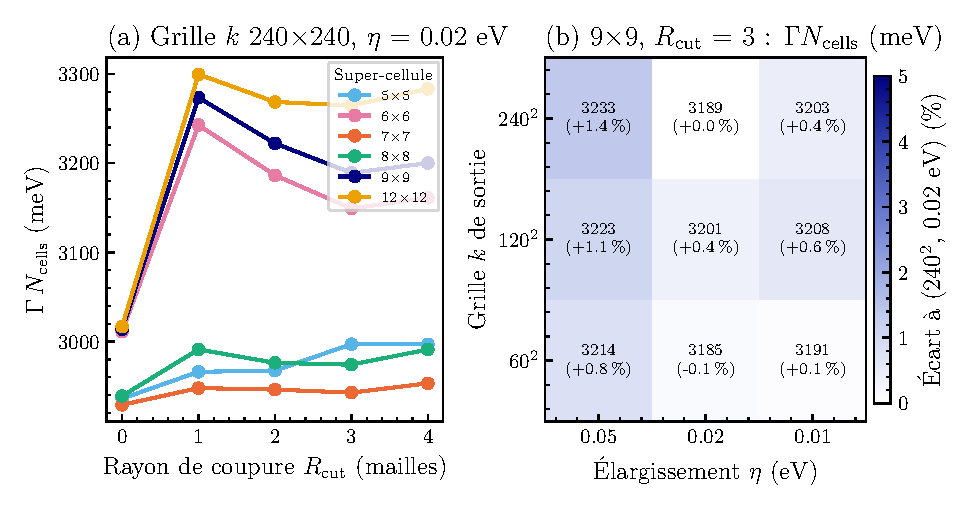
\includegraphics[width=\textwidth]{figures/fig_convergence.pdf}
    \caption[Convergence du taux d'amortissement par unité de
    concentration.]{Convergence de la médiane de $\Gamma N_\text{cells}$
    sur $\pm3$~eV autour de $E_D$. (a) En fonction du rayon de coupure
    $R_\text{cut}$ du schéma local pour les six tailles de super-cellule,
    avec une grille de sortie $240\times240$ et un élargissement $\eta = 20$~meV. (b) En fonction de la grille de sortie et de $\eta$, pour la super-cellule de référence $9\times9$ à $R_\text{cut} = 3$. La couleur donne l'écart au point $(240^2, 20~\text{meV})$. La grille interne est de $300\times300$ ($N_{\tilde\kv}=300^2$) dans tous les cas.}
    \label{fig:convergence}
\end{figure}
\begin{table}[htbp]
    \centering
    \caption[Convergence du taux d'amortissement en fonction du rayon de
    coupure.]{Médiane de $\Gamma\,N_\text{cells}$ (meV) sur $\pm3$~eV
    autour de $E_D$ en fonction du rayon de coupure $R_\text{cut}$, pour les
    six tailles de super-cellule (grille de sortie $240\times240$,
    $\eta = 20$~meV, grille interne $300\times300$). Nous distinguons les deux familles de super-cellules de la section~\ref{sec:M_détails}.}
    \label{tab:convergence_gamma}
    \begin{tabular}{c c ccccc}
        \hline\hline
        $N$ & $N \bmod 3$ & $R_\text{cut}=0$ & 1 & 2 & 3 & 4 \\
        \hline
        6  & 0 & 2611 & 2537 & 2512 & 2509 & --- \\
        9  & 0 & 2597 & 2489 & 2467 & 2474 & 2468 \\
        12 & 0 & 2585 & 2475 & 2454 & 2459 & --- \\
        \hline
        5  & 2 & 2628 & 2554 & 2534 & 2524 & --- \\
        7  & 1 & 2603 & 2508 & 2492 & 2487 & --- \\
        8  & 2 & 2598 & 2497 & 2475 & 2478 & --- \\
        \hline\hline
    \end{tabular}
\end{table}
Le comportement en $R_\text{cut}$ est le même pour toutes les tailles : le passage du site seul $R_\text{cut}=0$ à $R_\text{cut} =1$ abaisse le taux d'amortissement de 2.8 à 4.3~\%, celui de 1 à 2 de 1~\%, celui de 2 à 3 le modifie de moins de 0.4~\% et celui de 3 à 4 de 0.2~\% (calculé uniquement pour la super-cellule de référence). Le taux d'amortissement converge nettement plus vite en $R_\text{cut}$ que les éléments de matrice interpolés eux-mêmes (voir le tableau~\ref{tab:rcut_M}), pour lesquels l'écart à $R_\text{cut}=3$ est encore de 2 à 3~\%. Selon la figure~\ref{fig:convergence} (b), le doublement de la grille de sortie et la division de $\eta$ par deux changent la médiane de moins de 0.5~\%. Nous retenons donc $R_\text{cut}=3$, une grille de sortie de $N_{\kv_f}=240^2$ points, $\eta=20$ meV et une grille interne de $N_{\tilde\kv}=300^2$ points. La valeur de $R_\text{cut}=3$ offre en outre le meilleur compromis entre précision et coût : le passage à $R_\text{cut}=4$ multiplie par près de deux la dimension du sous-espace local pour un gain marginal de 0.2~\%. La grille interne, variée de $150^2$ à $600^2$ avec les paramètres de production fixés, change la médiane sur la fenêtre de moins de $0.2$~\% entre $300^2$ et $600^2$ et de $2.4$~\% sur la zone restreinte $|\varepsilon-E_D|\le0.3$ eV. La seule quantité sensible est le taux d'amortissement des états situés exactement au point de Dirac, surestimé de $5$~\% à $300^2$ et décroissant de façon monotone avec la densité de la grille interne : dans $\pm\eta$ autour de $E_D$, celle-ci ne contient que les points $K$ et $K'$ et l'échantillonnage y est marginal. Aucune quantité rapportée dans cette section ne repose sur ces seuls états. Chacun des paramètres retenus pour la production est au-delà du point où le taux d'amortissement cesse de varier à mieux que 0.5~\%.
\begin{figure}[htbp]
    \centering
    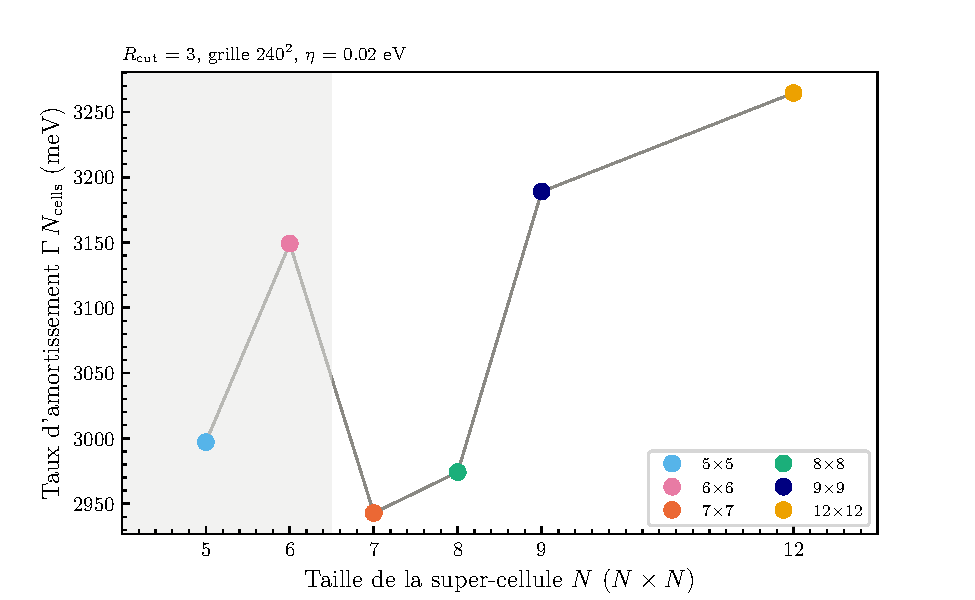
\includegraphics[width=\textwidth]{figures/fig_level2.pdf}
    \caption[Convergence du taux d'amortissement en taille de
    super-cellule.]{Médiane du taux d'amortissement $\Gamma N_\text{cells}$ sur $\pm3$~eV autour de $E_D$ en fonction de la taille $N$ de la super-cellule, avec
    les paramètres de production déterminés~: $R_\text{cut} = 3$, une grille de sortie de $240\times240$, un élargissement $\eta = 20$~meV et une grille interne de $300\times 300$. Les carrés représentent la famille avec $N$ divisible par trois ($N = 3m$) et les ronds représentent l'autre famille.}
    \label{fig:level2}
\end{figure}

Il reste la taille $N$ de la super-cellule, que nous examinons au sein de chaque famille de la section~\ref{sec:M_détails} dans la figure~\ref{fig:level2}. Il est évident que la convergence en taille de la super-cellule n'est pas atteinte, puisqu'aucun plateau n'est présent. Cependant, il y a une réduction régulière d'un facteur de $\sim 2$ par étape qui borne l'erreur de la référence $9\times9$ à $0.6$~\% par rapport à la super-cellule $12\times 12$, ce qui est suffisant pour les conclusions de ce chapitre. Il faudrait effectuer les calculs avec des super-cellules encore plus larges, ce que nous n'avons pas fait faute de temps et de ressources. Cette extension est laissée en perspective.

\newpage
\bloc{Tests du schéma local}

Le tableau~\ref{tab:tests_T} rassemble les vérifications du schéma local de la section~\ref{sec:T_détails}. Le test de référence compare le taux d'amortissement obtenu par le schéma local à celui de l'inversion directe de l'équation~\eqref{eqn:T_chap}, dans le même sous-espace des cinq fonctions de Wannier. Les deux coïncident à $5\times 10^{-14}$ pour $N=5$ et $\sim 10^{-9}$ pour $N=6, 12$. L'évaluation sur la grille d'énergie de pas $\eta/n_e$ introduit, par rapport à une grille quatre fois plus fine ($n_e = 32$), une erreur de $8\times 10^{-4}$ en médiane et de 1.5~\% au pire état. La médiane du taux d'amortissement sur la fenêtre ne change que de $3\times 10^{-4}$. Le taux est positif pour tous les états et $M_\text{loc}$ est hermitienne, comme l'imposent les contrôles. Comme à la section~\ref{sec:M_results}, ces tests établissent la cohérence interne de la méthode. Le contrôle externe vient de la comparaison avec la littérature, que nous effectuons plus bas.
\begin{table}[htbp]
    \centering
    \small
    \setlength{\tabcolsep}{4pt}
    \caption[Vérifications du schéma local.]{Vérifications de la chaîne
    de calcul local de la matrice $T$ et du taux d'amortissement : les tests et la quantité qu'ils contrôlent, la valeur obtenue et le seuil d'acceptation. Le test de
    référence compare le schéma local à l'inversion dense de
    l'équation~\eqref{eqn:T_chap} dans le sous-espace des cinq fonctions
    de Wannier. L'erreur de la grille d'énergie est mesurée par rapport à
    une grille quatre fois plus fine ($n_e = 32$), sur les états de la
    fenêtre $\pm3$~eV de la super-cellule référence $9\times9$. L'écart de la grille interne est mesuré entre $N_{\tilde\kv}=300^2$ et $600^2$ à paramètres de production fixés.}
    \label{tab:tests_T}
    \begin{tabular}{l l l l}
        \hline\hline
        Test & Quantité & Valeur & Seuil \\
        \hline
        Référence, $5\times5$ & $|\Gamma_\text{loc}-\Gamma_\text{dense}|/\Gamma$ & $5.1\times10^{-14}$ & $10^{-8}$ \\
        Référence, $6\times6$ & idem & $6.1\times10^{-9}$ & $10^{-8}$ \\
        Référence, $12\times12$ & idem & $3.7\times10^{-9}$ & $10^{-8}$ \\
        Grille d'énergie, $n_e = 8$ & $|\Delta\Gamma|/\Gamma$, méd. / p95 / max & $8\times10^{-4}$ / $5\times10^{-3}$ / $1.5\times10^{-2}$ & --- \\
        \quad sur la médiane de $\Gamma$ & écart relatif & $3\times10^{-4}$ & --- \\
        Grille interne, $300^2\to600^2$ & écart sur la médiane & $1.4\times10^{-3}$ & --- \\
        Hermiticité de $M_\text{loc}$ & $\max|M_\text{loc}-M_\text{loc}^\dagger|$ & $<10^{-10}$ & $10^{-10}$ \\
        Positivité & $\min\Gamma_{n\kv}$ & $\ge 0$ & $-10^{-8}$ \\
        \hline\hline
    \end{tabular}
\end{table}

\newpage
\bloc{Taux d'amortissement et approximation de Born}

\begin{figure}[htbp]
    \centering
    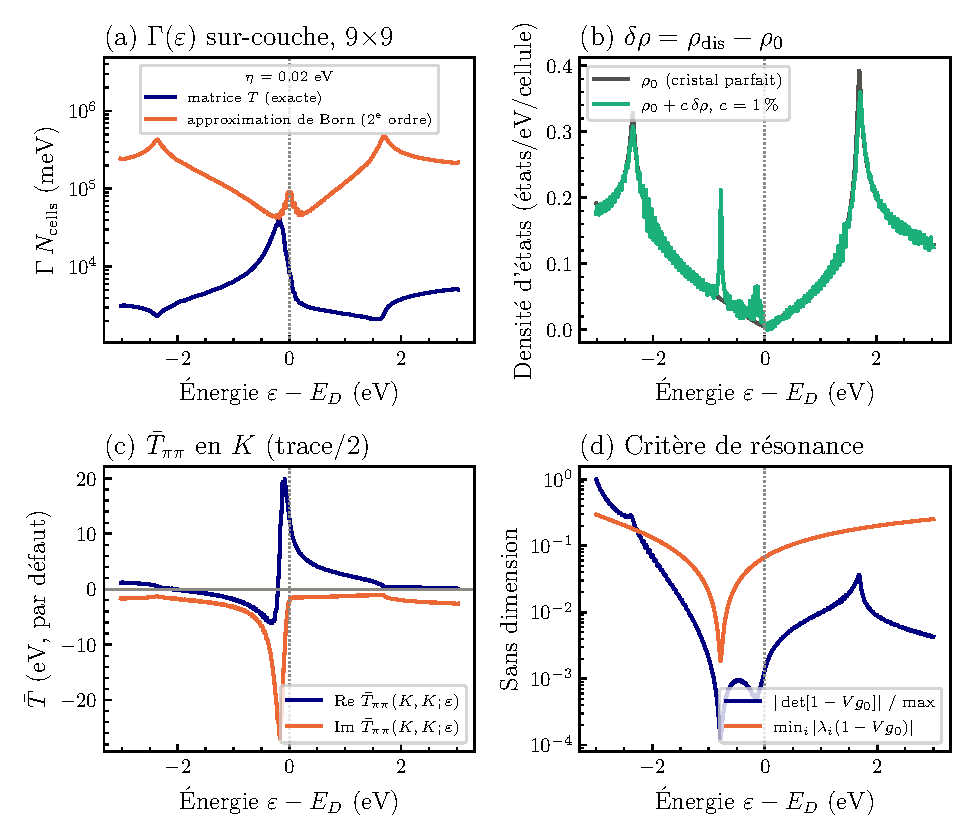
\includegraphics[width=\textwidth]{figures/fig_spectral_final.pdf}
    \caption[Taux d'amortissement et signatures spectrales d'une lacune
    dans le graphène.]{Taux d'amortissement et signatures spectrales d'une lacune dans le graphène, calculés pour la super-cellule de référence $9\times 9$ et les paramètres de production : $R_\text{cut}=3$, la grille de sortie $240\times 240$, un élargissement de $\eta=20$ meV et la grille interne de $300\times 300$. Les énergies sont mesurées à partir du point de Dirac $E_D$. (a) Taux d'amortissement sur couche $\Gamma N_\text{cells}$ des bandes $\pi$ et $\pi^*$ avec la matrice $T$ complète et l'approximation de Born, obtenu par la moyenne lorentzienne~\eqref{eqn:moyenne_lorentzienne} des taux individuels $\Gamma^\text{ed}_{n\kv}$ (b) Densité d'états du cristal parfait $\rho_0$ et pour une concentration de lacunes de $c=1~\%$, $\rho = \rho_0+c\delta\rho$. (c) Parties réelles et imaginaires de la quantité $\bar T(K;\varepsilon)$, définie comme la demi-trace sur la paire $\pi/\pi^*$ dégénérée en $K$, à l'image de $\bar M(K)$ de l'équation~\eqref{eqn:M_bar}. (d) Critère de résonance $\left|\det[\mathbb{I}-M_\text{loc}g^{(0)}(\varepsilon)]\right|$ normalisé et les plus petites valeurs propres de $\mathbb{I}-M_\text{loc}g^{(0)}$.}
    \label{fig:spectral}
\end{figure}
La figure~\ref{fig:spectral} (a) montre le taux d'amortissement $\Gamma N_\text{cells}$ des bandes $\pi$ et $\pi^*$, calculé avec la matrice $T$ complète et l'approximation de Born, pour les paramètres de production déterminés plus haut. Pour passer des taux individuels $\Gamma_{n\kv}^\text{ed}$, évalués chacun à leur propre énergie $\varepsilon_{n\kv}$, à une courbe continue en $\varepsilon$, nous prenons la moyenne lorentzienne normalisée
\begin{equation}
    \Gamma^\text{ed}(\varepsilon) = \frac{\sum_{n\kv}L_\eta(\varepsilon-\varepsilon_{n\kv})\Gamma^\text{ed}_{n\kv}}{\sum_{n\kv} L_\eta(\varepsilon-\varepsilon_{n\kv})},\qquad L_\eta(\varepsilon) = \frac{1}{\pi}\frac{\eta}{\varepsilon^2+\eta^2},\label{eqn:moyenne_lorentzienne}
\end{equation}
sur les états de la grille $240^2$ dans une fenêtre $|\varepsilon-E_D|\leq 3$ eV, avec $\eta=0.02$ eV. Le dénominateur est la densité d'états lisse et $\Gamma^\text{ed}(\varepsilon)$ est le taux d'amortissement moyen des états situés à moins de $\sim \eta$ de $\varepsilon$. Les médianes citées dans les tableaux de convergence sont prises sur les états eux-mêmes ; seule cette figure passe par la moyenne lorentzienne. À $c=1$~\%, le taux exact vaut $\sim 25$ meV en médiane sur la fenêtre de $\pm 3$ eV autour de $E_D$ et est maximal autour de $-1.2$~eV. L'approximation de Born surestime le taux exact d'un facteur de $3.3$ en médiane et jusqu'à $16$ au voisinage des singularités de van Hove, où elle diverge avec la densité d'états tandis que la matrice $T$ sature. C'est l'effondrement de l'approximation de Born pour un potentiel de défaut fort comme une lacune, tel que trouvé dans l'article de référence~\cite{kaasbjergAtomisticMatrixTheory2020}.

\newpage
\bloc{Signatures spectrales de la lacune}

Les panneaux (b-d) de la figure~\ref{fig:spectral} examinent la structure de la matrice $T$ elle-même. La quantité $\bar T(K;\varepsilon)$ au panneau (c), définie comme la demi-trace du bloc de la \textit{self}-énergie de la paire dégénérée à $K$, a une partie imaginaire minimale à $-1.3$ eV et un module maximal entre $-1.05$ et $-0.70$ eV. Les deux parties jouent des rôles distincts. C'est la partie imaginaire qui gouverne l'amortissement : son minimum coïncide avec le maximum de $\Gamma^\text{ed}$ au panneau (a), et non le maximum du module, situé quelque $0.3$ eV plus haut. La région de diffusion résonante est donc celle de la partie imaginaire. La partie réelle, elle, renormalise l'énergie des bandes ; elle porte la signature répulsive de la lacune et reste positive partout dans la fenêtre autour du point de Dirac. Le critère de pôle du panneau (d), qui localise les états liés et quasi-liés induits par le défaut, ne présente qu'une seule quasi-annulation à $\sim-2.5$~eV. La variation de densité d'états au panneau (b) confirme cet état : un pic étroit situé juste sous la singularité de van Hove de la bande $\pi$ à $\sim-2.5$~eV représente un état quasi-lié induit par la lacune, au sein du continuum de la bande. La règle de somme $\int\delta\rho\,d\varepsilon = 0$ sur toute la largeur de bande est satisfaite à moins de 0.06 état près. Au voisinage du point de Dirac, $\delta\rho$ ne présente qu'une faible structure.

\bloc{Comparaison avec la littérature}

Ces signatures se comparent à celles obtenues par Kaasbjerg~\cite{kaasbjergAtomisticMatrixTheory2020}, pour une lacune de carbone dans le graphène, qui trouve un état quasi-lié sous le point de Dirac à $c=1~\%$. L'accord est qualitatif seulement : le signe répulsif du potentiel, l'effondrement de l'approximation de Born et l'ordre de grandeur du taux d'amortissement sont en accord. Toutefois, la position exacte de l'état quasi-lié diffère : dans nos calculs, l'état dominant se trouve sous la singularité de van Hove plutôt qu'au voisinage du point de Dirac, où la littérature sur la monolacune du graphène situe le mode quasi-nul~\cite{pereiraDisorderInducedLocalized2006}, et où notre $\delta\rho$ n'a qu'un poids faible. Il est clair que la différence d'un facteur de $3$--$4$ entre nos éléments de matrice, qui se propage non linéairement au taux d'amortissement, a un impact sur cette comparaison quantitative. Nous n'avons pas pu lui attribuer une cause unique parmi la relaxation de la super-cellule défectueuse, le traitement des électrons de c\oe ur, la base d'ondes planes contre celle d'orbitales atomiques, la fonctionnelle d'échange-corrélation et l'approximation diagonale en bande de la matrice $T$ (section~\ref{sec:mbt_sigma}), que la référence n'effectue pas. De plus, nous avons relevé que notre taux n'est pas convergé par rapport à la taille de la super-cellule, ce qui a nécessairement un impact sur les propriétés spectrales de la lacune. Enfin, l'interpolation de la matrice de couplage dans le sous-espace des cinq fonctions de Wannier introduit une approximation : les états au-delà de la fenêtre externe, ainsi que la partie des bandes de haute énergie non capturée par le désenchevêtrement, sont absents de la base dans laquelle la matrice $T$ est construite. Nous nous attendons à ce que ces états ne contribuent pas significativement à la diffusion Raman résonante, mais cela constitue toutefois une différence réelle avec la base d'orbitales atomiques de la référence.

\section{Conclusion}
Ce chapitre a construit, à partir des premiers principes, une méthode complète pour le couplage électron-défaut, qui constitue la contribution originale centrale de ce mémoire. Les éléments de matrice $M_{mn}(\kv',\kv)$ sont définis à partir du potentiel induit par le défaut et séparés en une partie locale, évaluée dans l'espace réciproque~\eqref{eqn:ML_final}, et une partie non locale issue des projecteurs de Kleinman-Bylander~\eqref{eqn:MNL_final}. Deux idées centrales rendent notre méthode applicable au calcul de l'intensité Raman résonante sur des grilles ultra-denses. D'abord, le remplissage par zéros raffine la grille du potentiel de défaut et allège la contrainte de commensurabilité entre la super-cellule et la grille des fonctions de Wannier, ce qui nous permet d'obtenir la matrice de couplage sur des grilles relativement denses sans recourir à des calculs de super-cellules démesurés et intraitables. Ce remplissage par zéros rend par ailleurs manifeste la localisation des éléments de matrice de couplage dans la base de Wannier (section~\ref{sec:M_results}), ce qui autorise notre deuxième idée : l'interpolation par fonctions de Wannier, tronquée à un sous-espace local de petite dimension grâce à cette localisation, qui rend le calcul de la matrice $T$ praticable sur des grilles arbitrairement denses.

Nous avons appliqué notre méthode à une lacune non relaxée dans le graphène et ce chapitre livre trois résultats principaux. D'abord, l'échantillonnage de la zone de Brillouin sépare les super-cellules en deux familles selon que leur grille inclut ou non les points $K$ et $K'$ et nous prenons la super-cellule $9\times 9$, dont la grille les inclut, comme référence. Ensuite, le couplage est dominé par sa partie non locale, tandis que la partie locale, écrantée, porte toute la dépendance en taille de la super-cellule. Enfin, le taux d'amortissement par unité de concentration, obtenu dans le formalisme de la matrice $T$, révèle un état quasi-lié sous la singularité de van Hove de la bande $\pi$, plus profond que le mode quasi-nul attendu près du point de Dirac selon la littérature. L'approximation de Born surestime ce taux et diverge aux singularités de van Hove : pour un potentiel aussi intense que celui d'une lacune, la resommation de la matrice $T$ à tous les ordres en théorie de la perturbation est nécessaire. La chaîne de calcul est validée par une suite de tests systématiques, dont la reconstruction des valeurs propres de Kohn-Sham à quelques dizaines de $\mu$eV près.

Notre méthode souffre toutefois de plusieurs limitations. La géométrie autour du défaut n'est pas relaxée et la reconstruction de Jahn-Teller de la monolacune~\cite{el-barbaryStructureEnergeticsVacancy2003} est ignorée. Le taux d'amortissement n'est convergé qu'à $0.6$~\% entre les super-cellules $9\times 9$ et $12\times 12$, sans qu'un plateau soit atteint mais avec une décroissance régulière des écarts. Nos éléments de matrice calculés sont inférieurs d'un facteur de $3$--$4$ à ceux de Kaasbjerg~\cite{kaasbjergAtomisticMatrixTheory2020}, sans qu'une cause unique ait pu être isolée parmi la fonctionnelle d'échange-corrélation, la base d'ondes planes plutôt que d'orbitales atomiques, la relaxation autour du défaut, le traitement des électrons de c\oe ur, la troncature du sous-espace des fonctions de Wannier et l'approximation diagonale en bande de la matrice $T$. L'accord des éléments de matrice et des signatures spectrales reste toutefois qualitatif. La relaxation de la lacune, la généralisation à d'autres types de défauts, la convergence en taille de la super-cellule du taux d'amortissement, l'approximation de la matrice $T$ autocohérente au voisinage du point de Dirac~\cite{peresElectronicPropertiesDisordered2006}, ainsi que la structure matricielle en bande complète de la matrice $T$ sont laissées en perspective. De surcroît, nos calculs ne sont pas polarisés en spin, alors que la monolacune du graphène porte un moment magnétique local~\cite{yazyevDefectinducedMagnetismGraphene2007}. Un traitement polarisé, couplé à la relaxation de Jahn-Teller, modifierait la position de l'état quasi-lié et séparerait le taux d'amortissement en deux contributions de spin. Enfin, nous ne considérons qu'un seul type de défaut dans ce mémoire : les lacunes. La méthode est toutefois généralisable à n'importe quel type de défaut et cette généralisation est elle aussi laissée en perspective.

Le chapitre livre ainsi les deux quantités annoncées en introduction. Les éléments de matrice $M$ entrent directement dans les amplitudes de diffusion \textit{phonon-défaut} du chapitre~\ref{chap:Raman} et le taux d'amortissement $\Gamma^\text{ed}$ élargit les dénominateurs résonants de ces amplitudes. Pour les énergies d'excitation dans le visible typiquement utilisées dans les expériences de spectroscopie Raman, les états intermédiaires de la double résonance se situent précisément dans la fenêtre d'énergie où la diffusion sur la lacune est maximale et où l'approximation de Born échoue le plus~\cite{thomsenDoubleResonantRaman2000}. Le chapitre suivant calcule le second ingrédient de ces dénominateurs, le taux d'amortissement dû au couplage électron-phonon $\Gamma^\text{ep}$, et nous verrons que les deux contributions sont comparables dans cette fenêtre.